\chapter{Description of Formal Mathematics}

\section{TERMS AND RELATIONS}

\subsection{SIGNS AND ASSEMBLIES}

The signs of a mathematical theory \(\mathcal{C}\)\footnote{The meaning of this expression will become clear as the chapter progresses.} are the following :

\begin{enumerate}
\def\labelenumi{(\arabic{enumi})}
\item
  The logical signs\footnote{For the intuitive meanings of these signs, see no. 3, Remark.}: \(\square, \tau, \vee, \neg\).
\item
  The letters.
\end{enumerate}

By letters we mean upper and lower case Roman letters, with or without accents. Thus A, A', A'', A''', \ldots{} are letters. At any place in the text it is possible to introduce letters other than those which have appeared in previous arguments.

\begin{enumerate}
\def\labelenumi{(\arabic{enumi})}
\setcounter{enumi}{2}
\tightlist
\item
  The specific signs, which depend on the theory under consideration.
\end{enumerate}

In the theory of sets we shall use only the following three specific signs: \(=, \in, \supset\) .

An assembly in \(\mathfrak{C}\) is a succession of signs of \(\mathfrak{C}\) written next to one another; certain signs, other than letters, may be joined in pairs by bars above the line, which are called links. *For example, in the Theory of Sets, in which \(\in\) is a specific sign,

\pandocbounded{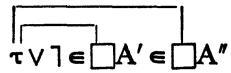
\includegraphics[keepaspectratio]{images/part001_434fa5c1de2e0e5711bd2657d8ea90475ca0e52e33fa2d57a405da317d612ec5.jpg}}

is an assembly.*

The exclusive use of assemblies would lead to insuperable difficulties both for the printer and for the reader. For this reason current texts use abbreviating symbols (notably words of ordinary speech) which do not belong to formal mathematics. The introduction of such symbols is the object of definitions. Their use is not indispensable to the theory, and can often lead to confusion which only a certain familiarity with the subject will enable the reader to avoid.

\minorheading{Examples}

\begin{enumerate}
\def\labelenumi{(\arabic{enumi})}
\item
  The assembly \(\vee\neg\) is represented by \(\Longrightarrow\) .
\item
  The following symbols represent assemblies (and very long ones at that):
\end{enumerate}

\[
\begin{gathered}
\text{``3 and 4''} \\
\phi \\
\mathbf{N} \\
\mathbf{Z} \\
\text{``the real line''} \\
\text{``the }\Gamma\text{ function''} \\
f \circ g \\
\pi = \sqrt{2} + \sqrt{3} \\
1 \in 2
\end{gathered}
\]

``Every finite division ring is a field''

``The zeros of \(\zeta(s)\) other than \(-2, -4, -6, \ldots\) lie on the line

\[
\mathcal{R}(s) = 1/2
\]''.

In general, the symbol used to represent an assembly contains all the letters which appear in the assembly. Nevertheless, this principle can sometimes be infringed without risk of confusion. *For example, ``the completion of X'' represents an assembly which contains the letter X, but which also contains the letter which represents the set of entourages of the uniform structure of X. On the other hand,

\[
\int_ {0} ^ {1} f (x) d x
\]

represents an assembly in which the letter x (and the letter d) do not appear; and the assemblies represented by N, Z, ``the Γ function'' do not contain any letters.*

A mathematical theory (or simply a theory) contains rules which allow us to assert that certain assemblies of signs are terms or relations of the theory, and other rules which allow us to assert that certain assemblies are theorems of the theory.

The description of these rules, which will appear in this chapter, does not belong to formal mathematics; the rules involve assemblies which are more or less undetermined, for example undetermined letters. To simplify the exposition it is convenient to denote such assemblies by less cumbersome symbols. We shall use, especially, combinations of signs (of a mathematical theory), bold-face italic letters (with or without indices or accents), and particular symbols, of which some examples will be given. Since our object is only to avoid circumlocutions (cf.~note (*), § 3, no. 1, p.~28) we shall not enunciate strict general rules for the use of these symbols; the reader will be able to reconstruct without trouble the assembly in question, in each particular case. By abuse of language we shall often say that the symbols are assemblies, rather than that they denote assemblies: expressions such as ``the assembly A'' or ``the letter x'', in the statements of the following rules, should therefore be replaced by ``the assembly denoted by A'' or ``the letter denoted by x''.

Let \(A\) and \(B\) be assemblies. We shall denote by \(AB\) the assembly obtained by writing the assembly \(B\) on the right of the assembly \(A\) . We shall denote by \(\vee A \neg B\) the assembly obtained by writing, from left to right, the sign \(\vee\) , the assembly \(A\) , the sign \(\neg\) , the assembly \(B\) . And so on.

Let \(A\) be an assembly and let \(x\) be a letter. We shall denote by \(\tau_{x}(A)\) the assembly constructed as follows: form the assembly \(\tau A\) , link each occurrence of \(x\) in \(A\) to the \(\tau\) written on the left of \(A\) , and then replace \(x\) everywhere it occurs by the sign \(\square\) . The assembly denoted by \(\tau_{x}(A)\) therefore does not contain \(x\) .

Example. The symbol \(\tau_{x}(\in xy)\) represents the assembly

\[
\tau \in \square y.
\]

Let A and B be assemblies and let x be a letter. The assembly obtained by replacing x, wherever it occurs in A, by the assembly B is denoted by \((B|x)A\) (read: B replaces x in A). If x does not appear in A, then \((B|x)A\) is identical with A; in particular,

\[
(B | \boldsymbol {x}) \tau_ {\boldsymbol {x}} (A)
\]

is identical with \(\tau_{\mathbf{x}}(A)\) .

Example. If we replace \(x\) by \(\square\) wherever \(x\) occurs in the assembly \(\vee \in xy = xx\) , we obtain the assembly \(\vee \in \square y = \square \square\) .

If \(A\) is an assembly and we are interested particularly in a letter \(x\) , or two distinct letters \(x\) and \(y\) (which may or may not appear in \(A\) ), we shall often write \(A \{x\}\) or \(A \{x, y\}\) . In this case we write \(A \{B\}\) instead of \((B|x)A\) . We denote by \(A \{B, C\}\) the assembly obtained by simultaneously replacing \(x\) by \(B\) and \(y\) by \(C\) wherever they occur in \(A\) (note that \(x\) and \(y\) may appear in \(B\) and in \(C\) ); if \(x'\) and \(y'\) are distinct letters, other than \(x\) and \(y\) , which appear in neither \(A, B\) , nor \(C\) , then \(A \{B, C\}\) is the same as \((B|x') (C|y') (x'|x) (y'|y)A\) .

Remark. When an abbreviating symbol \(\Sigma\) is introduced, by means of a definition, to represent a certain assembly, the (usually tacit) convention is made of representing the assembly obtained by substituting an assembly B for a letter x in the original assembly, by the symbol obtained by the replacing the letter x in \(\Sigma\) by the assembly B (or, more often, by an abbreviating symbol representing the assembly B).

¶ *For example, having defined what assembly is represented by the symbol E⊗F, where E and F are letters --- an assembly which, incidentally, contains other letters besides E and F --- the symbol Z⊗F can be used without further explanation.*

¶ This rule can lead to confusions, which are avoided by the use of various typographical devices; the most common consists in replacing x by (B) in place of B.

¶ *For example, M∩N denotes an assembly containing the letter N. If we substitute for N the assembly represented by P∪Q, we get an assembly denoted by M∩(P∪Q).*

\subsection{CRITERIA OF SUBSTITUTION}

Formal mathematics contains only explicitly written assemblies. Nevertheless, even with the use of abbreviating symbols, the development of mathematics strictly in accordance with this principle would lead to extremely long chains of reasoning. For this reason we shall establish criteria relating to indeterminate assemblies; each of these criteria will describe once for all the final result of a definite sequence of manipulations on these assemblies. These criteria are therefore not indispensable to the theory; their justification belongs to metamathematics.

The development of metamathematics itself requires, in practice, the use of abbreviating symbols, some of which have already been indicated. Most of these symbols are also used in mathematics.

We shall make use of the following criteria, called the criteria of substitution:

CS1. Let A and B be assemblies and let x and \(x'\) be letters. If \(x'\) does not appear in A, then \((B|x)A\) is identical with \((B|x')(x'|x)A\) .

CS2. Let \(A, B\) , and \(C\) be assemblies and let \(x\) and \(y\) be distinct letters\footnote{In accordance with what was said in no. 1, the phrase ``x and y are distinct letters'' is an abuse of language: it means that x and y denote distinct letters in the assemblies under consideration.}. If \(y\) does not appear in \(B\) , then \((B|x)(C|y)A\) is identical with

\[
\left(\boldsymbol {C} ^ {\prime} | \boldsymbol {y}\right) (\boldsymbol {B} | \boldsymbol {x}) \boldsymbol {A},
\]

where \(C'\) is the assembly \((B|x)C\) .

CS3. Let A be an assembly and let x and \(x'\) be letters. If \(x'\) does not appear in A, then \(\tau_{\mathbf{x}}(A)\) is identical with \(\tau_{\mathbf{x}'}(A')\) , where \(A'\) is the assembly \((x'|x)A\) .

CS4. Let A and B be assemblies and let x and y be distinct letters. If x does not appear in B, then \((B|y)\tau_{x}A\) is identical with \(\tau_{x}(A')\) , where \(A'\) is the assembly \((B|y)A\) .

CS5. Let \(A, B, C\) be assemblies and let \(x\) be a letter. The assemblies \((C|x) (\neg A), (C|x) (\vee AB), (C|x) (\Longrightarrow AB), (C|x) (sAB)\) (where \(s\) is a specific sign) are respectively identical with \(\neg A', \vee A'B', \Longrightarrow A'B', sA'B',\) where \(A', B'\) are respectively \((C|x) A, (C|x) B\) .

As an example, let us indicate the principle of the verification of CS2. Compare the operation which takes us from A to \((B|x)(C|y)A\) with the operation which takes us from A to \((C'|y)(B|x)A\) . In each operation, no sign which appears in A and is distinct from x and y is altered. At every place where x appears in A, we have to substitute B for x in the first and in the second operation; this is clear in regard to the first operation, and in regard to the second it follows from the fact that y does not appear in B. Finally, at every place where y appears in A, the first operation consists in replacing C for y, then B for x at every place where x appears in C; but it is clear that this comes to the same thing as substituting for y, wherever it appears in A, the assembly \((B|x)C\) .

\subsection{FORMATIVE CONSTRUCTIONS}

Some of the specific signs of a theory are called relational, and the others are called substantific. With every specific sign is associated a natural number called its weight (which is practically always the number 2).

¶ An assembly is said to be of the first species if it begins with a τ, or with a substantific sign, or if it consists of a single letter; otherwise it is of the second species.

¶ A formative construction in a theory \(\mathfrak{C}\) is a sequence of assemblies which has the following property: for each assembly A of the sequence, one of the following conditions is satisfied:

\begin{enumerate}
\def\labelenumi{(\alph{enumi})}
\item
  A is a letter.
\item
  There is in the sequence an assembly B of the second species, preceding A, such that A is \(\neg B\) .
\item
  There are two assemblies \(\pmb{B}\) and \(\pmb{C}\) of the second species (distinct or not), preceding \(\pmb{A}\) , such that \(\pmb{A}\) is \(\vee \pmb{BC}\) .
\item
  There is an assembly B of the second species, preceding A, and a letter x such that A is \(\tau_{x}(B)\) .
\item
  There is a specific sign \(s\) of weight \(n\)\footnote{As was said above, it would be possible, for the development of present-day mathematical theories, to limit our consideration to specific signs of weight 2, and consequently to avoid using the expression ``natural number n'' in the definition of a formative construction.} in \(\mathfrak{C}\) , and \(n\) assemblies \(A_{1}, A_{2}, \ldots, A_{n}\) of the first species, preceding \(A\) , such that \(A\) is \(sA_{1}A_{2} \ldots A_{n}\) .
\end{enumerate}

¶ The assemblies of the first species (resp. of the second species) which appear in the formative constructions of \(\mathfrak{C}\) are called terms (resp. relations) in \(\mathfrak{C}\).

Example. *In the theory of sets, in which \(\in\) is a relational sign of weight 2, the following sequence of assemblies is a formative construction :

\pandocbounded{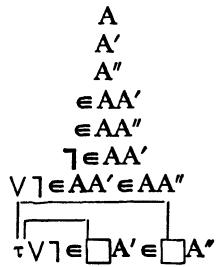
\includegraphics[keepaspectratio]{images/part001_f4a426ee2f8fe397dc0bc6599464a758ff3a832b6925cc474c9242d7de093d2f.jpg}}

Hence the assembly given as an example in no. 1 is a term in the theory of sets.*

Remark. Intuitively, terms are assemblies which represent objects, and relations are assemblies which represent assertions which can be made about these objects. Condition (a) means that the letters represent objects. Condition (b) means that if B is an assertion, then \(\neg B\) , called the negation of B, is an assertion (which is read: not B). Condition (c) means that if B and C are assertions, \(\vee BC\) , which is called the disjunction of B and C, is an assertion (which is read: either B or C); thus \(\Longrightarrow BC\) is an assertion (in words: ``either not B, or C'', or ``B implies C''). Condition (d) means that if B is an assertion and x a letter, then \(\tau_{X}(B)\) is an object. Let us consider the assertion B as expressing a property of the object X; then, if there exists an object which has the property in question, \(\tau_{X}(B)\) represents a distinguished object which has this property; if not, \(\tau_{X}(B)\) represents an object about which nothing can be said. Finally, condition (e) means that if \(A_{1}, A_{2}, ..., A_{n}\) are objects, and if s is a relational (resp. substantific) sign of weight n, then \(sA_{1}A_{2}\ldots A_{n}\) is an assertion about the objects \(A_{1}, ..., A_{n}\) (resp. an object depending on \(A_{1}, ..., A_{n}\) ).

Examples. The symbols \(\phi\) , \(\mathbf{N}\) , ``the real line'', ``the \(\Gamma\) function'', \(f \circ g\) represent terms. The symbols \(\pi = \sqrt{2} + \sqrt{3}\) , \(1 \in 2\) , ``every finite division ring is a field'', ``the zeros of \(\zeta(s)\) other than \(-2, -4, -6, \ldots\) lie on the line \(\mathcal{R}(s) = 1/2\)'' represent relations. The symbol ``3 and 4'' represents neither a term nor a relation.

The initial sign of a relation is \(\vee, \neg\) , or a relational sign. The initial sign of a term is either \(\tau\) or a substantific sign, provided that the term does not consist of a single letter. The latter assertion follows from the fact that a term is an assembly of the first species. If \(A\) is a relation, then \(A\) features in a formative construction, is not a letter, and does not begin with \(\tau\) , so that three cases are possible: (1) \(A\) is preceded by an assembly \(B\) such that \(A\) is \(\neg B\) ; (2) \(A\) is preceded by two assemblies \(B\) and \(C\) such that \(A\) is \(\vee BC\) ; (3) \(A\) is preceded by assemblies \(A_1, A_2, ..., A_n\) such that \(A\) is \(sA_1A_2 ... A_n\) , \(s\) being a relational sign.

\subsection{FORMATIVE CRITERIA}

CF1. If \(A\) and \(B\) are relations in a theory \(\mathfrak{G}\) , then \(\vee AB\) is a relation in \(\mathfrak{G}\) .

Consider two formative constructions (in \(\mathfrak{G}\) ), one of which contains \(A\) and the other \(B\) . Consider the sequence of assemblies obtained by writing first the assemblies of the first construction, then the assemblies of the second construction, and finally \(\vee AB\) . Since \(A\) and \(B\) are of the second species, it is immediately verified that this sequence is a formative construction of \(\mathfrak{G}\) . The assembly \(\vee AB\) is of the second species, hence it is a relation in \(\mathfrak{G}\) .

The three following criteria are established similarly:

CF2. If A is a relation in a theory C, then \(\neg A\) is a relation in C.

CF3. If A is a relation in a theory G, and if x is a letter, then \(\tau_{x}(A)\) is a term in G.

CF4. If \(A_1, A_2, \ldots, A_n\) are terms in a theory \(\mathfrak{C}\) , and if \(s\) is a relational (resp. substantific) sign of weight \(n\) in \(\mathfrak{C}\) , then \(sA_1A_2\ldots A_n\) is a relation (resp. a term) in \(\mathfrak{C}\) .

These criteria immediately imply the following :

CF5. If A and B are relations in a theory C, then \(\Longrightarrow AB\) is a relation in C.

CF6. Let \(A_1, A_2, \ldots, A_n\) be a formative construction in a theory \(\mathfrak{C}\) , and let \(x\) and \(y\) be letters. Suppose that \(y\) does not appear in any \(A_i\) . Then \((y|x)A_1\) , \((y|x)A_2, \ldots, (y|x)A_n\) is a formative construction in \(\mathfrak{C}\) .

To prove CF6, let \(A_i'\) be the assembly \((y|x)A_i\) . If \(A_i\) is a letter, then \(A_i'\) is a letter. If \(A_i\) is of the form \(\neg A_j\) , where \(A_j\) is an assembly of the second species which precedes \(A_i\) in the construction, then \(A_i'\) is identical with \(\neg A_j'\) by CS5, and \(A_j'\) is an assembly of the second species. The reasoning is similar if \(A_i\) is of the form \(\vee A_jA_k\) or \(sA_{j_1}A_{j_2}\ldots A_{j_m}\) , \(s\) being a specific sign of \(\mathfrak{G}\) . If finally \(A_i\) is of the form \(\tau_z(A_j)\) , where \(A_j\) is an assembly of the second species which precedes \(A_i\) ; in the construction, there are various cases to consider:

\begin{enumerate}
\def\labelenumi{(\alph{enumi})}
\item
  z is a letter distinct from x and y. Then \(A_{i}^{\prime}\) is identical with \(\tau_{z}(A_{j}^{\prime})\) by CS4, and \(A_{j}^{\prime}\) is an assembly of the second species.
\item
  z is identical with x. Then \(A_{i}\) does not contain x, hence \(A_{i}^{\prime}\) is identical with \(A_{i}\) , that is to say with \(\tau_{x}(A_{j})\) ; since y does not appear in \(A_{j}\) , \(\tau_{x}(A_{j})\) is identical with \(\tau_{y}(A_{j})\) by CS3.
\item
  z is identical with y. Then \(A_{i}\) is the assembly \(\tau A_{j}\) , because y does not appear in \(A_{j}\) ; therefore \(A_{i}^{\prime}\) is the assembly \(\tau A_{j}^{\prime}\) , that is \(\tau_{u}(A_{j}^{\prime})\) , where u is a letter which does not appear in \(A_{j}^{\prime}\) .
\end{enumerate}

CF7. Let \(A\) be a relation (resp. a term) in a theory \(\mathfrak{G}\) , and let \(x\) and \(y\) be letters. Then \((y|x)A\) is a relation (resp. a term) in \(\mathfrak{G}\) .

Let \(A_1, A_2, \ldots, A_n\) be a formative construction in which \(A\) appears. We shall show step by step that, if \(A_t\) is a relation (resp. a term) then \((y|x)A_t\) , which we shall denote by \(A_t'\) , is also a relation (resp. a term). Suppose that this point has been established for \(A_1, A_2, \ldots, A_{i-1}\) ; let us prove it for \(A_i\) . If \(A_i\) is a letter, then \(A_i'\) is a letter. If \(A_i\) is preceded in the construction by a relation \(A_j\) such that \(A_i\) is \(\neg A_j\) , then \(A_i'\) is identical with \(\neg A_j'\) by CS5, and \(\neg A_j'\) is a relation by CF2. The argument is similar if \(A_i\) is preceded by relations \(A_j, A_k\) such that \(A_i\) is \(\vee A_jA_k\) , or if \(A_i\) is preceded by terms \(A_{j_1}, \ldots, A_{j_m}\) such that \(A_i\) is \(sA_{j_1}\ldots A_{j_m}\) , where \(s\) is a specific sign of \(\mathfrak{G}\) of weight \(m\) . Finally, if \(A_i\) is preceded by a relation \(A_j\) such that \(A_i\) is \(\tau_z(A_j)\) , there are various cases to consider:

\begin{enumerate}
\def\labelenumi{(\alph{enumi})}
\item
  z is distinct from both x and y. Then \(A_{i}^{\prime}\) is identical with \(\tau_{\mathbf{z}}(A_{j}^{\prime})\) by CS4, and we know already that \(A_{j}^{\prime}\) is a relation; hence \(A_{i}^{\prime}\) is a term, by CF3.
\item
  \(z\) is identical with \(x\) . Then \(A_i\) does not contain \(x\) , therefore \(A_i'\) is identical with \(A_i\) , and consequently is a term.
\item
  \(z\) is identical with \(y\) . Then let \(u\) be a letter, distinct from both \(x\) and \(y\) , which does not appear in \(A_1, A_2, \ldots, A_j\) . By CF6, the sequence of assemblies \((u|y) A_1, \ldots, (u|y) A_j\) , which we shall denote by \(A_1'', \ldots, A_j''\) , constitutes a formative construction in \(\mathfrak{G}\) . Since \(y\) no longer appears in this new construction, \((y|x) A_1'', \ldots, (y|x) A_j''\) is a formative construction by CF6, so that \((y|x) A_j''\) is a relation in \(\mathfrak{G}\) ; consequently \(\tau_u((y|x)A_j'')\)
\end{enumerate}

is a term of \(\mathfrak{C}\) . But this term is identical with \((y|x)\tau_u(A_j'')\) by CS4, hence with \((y|x)\tau_y(A_j)\) by CS3, hence is identical with \(A_i'\) .

CF8. Let \(A\) be a relation (resp. a term) in a theory \(\mathfrak{G}\) , let \(x\) be a letter and \(T\) a term in \(\mathfrak{G}\) . Then \((T|x)A\) is a relation (resp. a term) in \(\mathfrak{G}\) .

Let \(A_1, A_2, \ldots, A_n\) be a formative construction in which \(A\) appears. Let \(x_1, x_2, \ldots, x_p\) be the distinct letters which appear in \(T\) . Let us associate with each letter \(x_i\) a letter \(x_i'\) , distinct from each of the letters \(x_1, \ldots, x_p\) and the letters which appear in \(A_1, \ldots, A_n\) , in such a way that the letters \(x_1', \ldots, x_p'\) are all distinct. The assembly

\[
\left(\boldsymbol {x} _ {1} ^ {\prime} \mid \boldsymbol {x} _ {1}\right) \left(\boldsymbol {x} _ {2} ^ {\prime} \mid \boldsymbol {x} _ {2}\right) \dots \left(\boldsymbol {x} _ {p} ^ {\prime} \mid \boldsymbol {x} _ {p}\right) \boldsymbol {T}
\]

is a term \(\pmb{T}'\) by CF7, and \((\pmb{T}|\pmb{x})\pmb{A}\) is identical with

\[
\left(\boldsymbol {x} _ {1} \mid \boldsymbol {x} _ {1} ^ {\prime}\right) \left(\boldsymbol {x} _ {2} \mid \boldsymbol {x} _ {2} ^ {\prime}\right) \dots \left(\boldsymbol {x} _ {p} \mid \boldsymbol {x} _ {p} ^ {\prime}\right) \left(\boldsymbol {T} ^ {\prime} \mid \boldsymbol {x}\right) \boldsymbol {A}
\]

by application of CS1. It is therefore enough to show that \((T^{\prime}|x)A\) is a relation (resp. a term); in other words, we may suppose from now on that the letters which appear in \(T\) do not appear in \(A_{1},\ldots ,A_{n}\) . We shall show step by step that, if \(A_{t}\) is a relation (resp. a term), then \((T|x)A_{t}\) , which we shall denote by \(A_{t}^{\prime}\) , is a relation (resp. a term). Suppose this point has been established for \(A_{1},A_{2},\ldots ,A_{i - 1}\) , and let us prove it for \(A_{i}\) . If \(A_{i}\) is a letter, then \(A_{i}^{\prime}\) is either the same letter or \(T\) , and therefore a term. If \(A_{i}\) is of the form \(\lnot A_j\) , where \(A_{j}\) is a relation which precedes \(A_{i}\) in construction, then \(A_{i}^{\prime}\) is identical with \(\lnot A_j^{\prime}\) by CS5, and we know already that \(A_{j}^{\prime}\) is a relation, hence \(A_{i}^{\prime}\) is a relation by CF2. The proof is analogous if \(A_{i}\) is of the form \(\vee A_{j}A_{k}\) , or \(sA_{j_1}\ldots A_{j_m}\) . Finally, if \(A_{i}\) is of the form \(\tau_{z}(A_j)\) , where \(A_{j}\) is a relation which precedes \(A_{i}\) in the construction, there are various cases to be considered:

\begin{enumerate}
\def\labelenumi{(\alph{enumi})}
\item
  \(z\) is distinct from \(x\) and from the letters which appear in \(T\) . Then \(A_i'\) is identical with \(\tau_z(A_j')\) by CS4, and we know already that \(A_j'\) is a relation; hence \(A_i'\) is a term by CF3.
\item
  \(\pmb{z}\) is identical with \(\pmb{x}\) . Then \(A_{i}\) does not contain \(\pmb{x}\) , hence \(A_{i}'\) is identical with \(A_{i}\) and consequently is a term.
\item
  \(z\) appears in \(T\) . Then \(z\) does not appear in \(A_j\) , so that \(A_i'\) is identical with \(\tau A_j\) ; hence \(A_i'\) is identical with \(\tau A_j'\) . Now, we know already that \(A_j'\) is a relation, and \(\tau A_j'\) is identical with \(\tau_u(A_j')\) , where \(u\) is a letter which does not appear in \(A_j'\) ; it follows by CF3 that \(A_i'\) is a term.
\end{enumerate}

Intuitively, if A is a relation in C, which we may regard as expressing a property of an object x, the assertion \((B|x)A\) amounts to saying that the object B has this property. If A is a term in C, it represents an object which depends in some way on the object denoted by x; the term \((B|x)A\) represents what the object A becomes when we take x to be the object B.

\section{THEOREMS}

From now on, if \(A\) is a relation, we shall write not(A) instead of \(\neg A\) . If \(A\) and \(B\) are relations, we shall write ``(A) or (B)'' instead of \(\vee AB\) , and \((A) \Longrightarrow (B)\) instead of \(\Longrightarrow AB\) . Sometimes we shall leave out the brackets. In each case the reader will be able to determine without difficulty the assembly under consideration.

\subsection{AXIOMS}

We have already seen that the specific signs determine the terms and the relations in a theory \(\mathfrak{G}\) . To construct \(\mathfrak{G}\) , we proceed as follows:

\begin{enumerate}
\def\labelenumi{(\arabic{enumi})}
\item
  First we write down a certain number of relations in \(\mathfrak{G}\) ; these are called the explicit axioms of \(\mathfrak{G}\) . The letters which appear in the explicit axioms are called the constants of \(\mathfrak{G}\) .
\item
  We lay down one or more rules\footnote{For the sake of brevity, these rules are expressed by using the symbols mentioned in §1, no. 1 (and especially bold-faced italic letters); but it would be easy to avoid the use of these symbols completely in the formulation of the rules (see §3, no. 1, note (*) on p. 28).}, called the schemes of \(\mathfrak{C}\) , which must have the following properties: (a) the application of such a rule \(\mathcal{R}\) furnishes a relation in \(\mathfrak{C}\) ; (b) if \(T\) is a term in \(\mathfrak{C}\) , if \(x\) is a letter, and if \(R\) is a relation in \(\mathfrak{C}\) constructed by applying the scheme \(\mathcal{R}\) , then the relation \((T|x)R\) can also be constructed by applying \(\mathcal{R}\) .
\end{enumerate}

In all the cases we envisage, the verification of these conditions is always easy.

Every relation constructed by applying a scheme of \(\mathfrak{G}\) is called an implicit axiom of \(\mathfrak{G}\) .

Intuitively, the axioms represent either self-evident assertions or else hypotheses from which one wishes to draw consequences. The constants represent well-defined objects for which the properties expressed by the explicit axioms are supposed to be true. On the other hand, if the letter x is not a constant, it represents a completely undetermined object; if a property of the object x is assumed to be true by means of an axiom, then this axiom is necessarily implicit, so that the property remains true for any object T.

\subsection{PROOFS}

A demonstrative text in a theory \(\mathfrak{G}\) comprises:

\begin{enumerate}
\def\labelenumi{(\arabic{enumi})}
\item
  An auxiliary formative construction of relations and terms in \(\mathfrak{G}\) .
\item
  A proof in \(\mathfrak{G}\) , that is to say a sequence of relations in \(\mathfrak{G}\) which appear in the auxiliary formative construction, such that for every relation \(\pmb{R}\) in the sequence at least one of the following conditions is satisfied:
\end{enumerate}

\((a_{1})\boldsymbol{R}\) is an explicit axiom of \(\mathfrak{c}\) .

\((a_{2})\) R results from the application of a scheme of C to terms or relations which appear in the auxiliary formative construction.

\begin{enumerate}
\def\labelenumi{(\alph{enumi})}
\setcounter{enumi}{1}
\tightlist
\item
  there are two relations \(S, T\) in the sequence which precede \(R\) , such that \(T\) is \(S \Longrightarrow R\) .
\end{enumerate}

¶ A theorem in \(\mathfrak{G}\) is a relation which appears in a proof in \(\mathfrak{G}\).

This notion is therefore essentially dependent on the state of the theory under consideration, at the time when it is being described. A relation in a theory \(\mathfrak{G}\) becomes a theorem in \(\mathfrak{G}\) when one succeeds in inserting it into a proof in \(\mathfrak{G}\) . To say that a relation in \(\mathfrak{G}\) ``is not a theorem in \(\mathfrak{G}\)'' cannot have any meaning without reference to the stage of development of the theory \(\mathfrak{G}\) .

A theorem in \(\mathfrak{G}\) is also called a ``true relation in \(\mathfrak{G}\) '' (or ``proposition'', ``lemma'', ``corollary'', etc.). Let \(R\) be a relation in \(\mathfrak{G}\) , let \(x\) be a letter and \(T\) a term in \(\mathfrak{G}\) ; if \((T|x)R\) is a theorem in \(\mathfrak{G}\) , \(T\) is said to satisfy the relation \(R\) in \(\mathfrak{G}\) (or to be a solution of \(R\) ), when \(R\) is considered as a relation in \(x\) .

A relation is said to be false in \(\mathfrak{c}\) if its negation is a theorem in \(\mathfrak{c}\) . A theory \(\mathfrak{c}\) is said to be contradictory when one has written a relation which is both true and false in \(\mathfrak{c}\) .

Here again, we are dealing with a notion that depends on the particular state of development of a theory. The reader should beware of the confusion (unfortunately suggested by the intuitive meaning of the word ``false'') which consists in believing that, once one has proved that a relation R is false in \(\mathfrak{G}\) , one has thereby established that R ``is not true'' in \(\mathfrak{G}\) (strictly speaking, this phrase has no precise meaning in mathematics, as we have remarked above).

¶ In what follows we shall give metamathematical criteria, called deductive criteria, which will allow us to shorten proofs. These criteria will be denoted by the letter C followed by a number.

C1 (Syllogism). Let A and B be relations in a theory C. If A and \(A \Longrightarrow B\) are theorems in C, then B is a theorem in C.

Let \(R_1, R_2, \ldots, R_n\) be a proof in \(\mathfrak{G}\) in which \(A\) appears, and let \(S_1, S_2, \ldots, S_p\) be a proof in \(\mathfrak{G}\) in which \(A \Longrightarrow B\) appears. Clearly \(R_1, R_2, \ldots, R_n, S_1, S_2, \ldots, S_p\) is a proof in \(\mathfrak{G}\) in which both \(A\) and \(A \Longrightarrow B\) appear. Hence

\[
\boldsymbol {R} _ {1}, \boldsymbol {R} _ {2}, \dots , \boldsymbol {R} _ {n}, \boldsymbol {S} _ {1}, \boldsymbol {S} _ {2}, \dots , \boldsymbol {S} _ {p}, \boldsymbol {B}
\]

is a proof in \(\mathfrak{c}\) , and therefore \(\pmb{B}\) is a theorem in \(\mathfrak{c}\) .

\subsection{SUBSTITUTIONS IN A THEORY}

Let \(\mathfrak{c}\) be a theory, let \(A_{1}, A_{2}, \ldots, A_{n}\) be its explicit axioms, let \(\pmb{x}\) be a letter and \(\pmb{T}\) a term of \(\mathfrak{c}\) . Let \((\pmb{T}|\pmb{x})\mathfrak{c}\) be the theory whose signs and schemes are the same as those of \(\mathfrak{c}\) , and whose explicit axioms are \((\pmb{T}|\pmb{x})\pmb{A}_{1}, (\pmb{T}|\pmb{x})\pmb{A}_{2}, \ldots, (\pmb{T}|\pmb{x})\pmb{A}_{n}\) .

C2. Let A be a theorem in a theory \(\mathfrak{G}\) , let T be a term of \(\mathfrak{G}\) , and let x be a letter. Then \((T|x)A\) is a theorem in the theory \((T|x)\mathfrak{G}\) .

Let \(R_1, R_2, \ldots, R_n\) be a proof in \(\mathfrak{G}\) in which \(A\) appears. Consider the sequence \((T|x)R_1, (T|x)R_2, \ldots, (T|x)R_n\) , which is a sequence of relations in \(\mathfrak{G}\) by reason of CF8 (§ 1, no. 4). We shall show that this sequence is a proof in the theory \((T|x)\mathfrak{G}\) ; this will establish the criterion. If \(R_k\) is an implicit axiom of \(\mathfrak{G}\) , then \((T|x)R_k\) is again an implicit axiom of \(\mathfrak{G}\) (no. 1) and therefore of \((T/x)\mathfrak{G}\) . If \(R_k\) is an explicit axiom of \(\mathfrak{G}\) , then \((T|x)R_k\) is an explicit axiom of \((T|x)\mathfrak{G}\) . Finally, if \(R_k\) is preceded by relations \(R_i\) and \(R_j\) , where \(R_j\) is \(R_i \Longrightarrow R_k\) , then \((T|x)R_k\) is preceded by \((T|x)R_i\) and \((T|x)R_j\) , and the latter is identical with \((T|x)R_i \Longrightarrow (T|x)R_k\) (criterion CS5).

C3. Let A be a theorem of a theory G, let T be a term of G, and let x be a letter which is not a constant of G. Then \((T|x)A\) is a theorem of G.

This follows immediately from C2, because x does not feature in the explicit axioms of \(\mathfrak{G}\). More particularly, if \(\mathfrak{G}\) contains no explicit axioms, or if the explicit axioms contain no letters, then the criterion C3 applies without restriction on the letter x.

\subsection{COMPARISON OF THEORIES}

A theory \(\mathcal{C}'\) is said to be stronger than a theory \(\mathcal{C}\) if all the signs of \(\mathcal{C}\) are signs of \(\mathcal{C}'\) , all the explicit axioms of \(\mathcal{C}\) are theorems in \(\mathcal{C}'\) , and the schemes of \(\mathcal{C}\) are schemes of \(\mathcal{C}'\) .

C4. If a theory \(\mathfrak{G}'\) is stronger than a theory \(\mathfrak{G}\) , then all the theorems of \(\mathfrak{G}\) are theorems of \(\mathfrak{G}'\) .

Let \(R_1, R_2, \ldots, R_n\) be a proof in \(\mathfrak{G}\) . We shall show, step by step, that each \(R_i\) is a theorem in \(\mathfrak{G}'\) . Suppose that this is true for the relations preceding \(R_k\) . If \(R_k\) is an axiom of \(\mathfrak{G}\) , it is a theorem in \(\mathfrak{G}'\) by hypothesis. If \(R_k\) is preceded by relations \(R_i\) and \(R_i \Longrightarrow R_k\) , we know already that \(R_i\) and \(R_i \Longrightarrow R_k\) are theorems in \(\mathfrak{G}'\) , and therefore \(R_k\) is a theorem in \(\mathfrak{G}'\) by virtue of C1. Hence, in every case, \(R_k\) is a theorem in \(\mathfrak{G}'\) , and the proof is complete.

If each of two theories \(\mathfrak{G}\) and \(\mathfrak{G}'\) is stronger than the other, \(\mathfrak{G}\) and \(\mathfrak{G}'\) are said to be equivalent. Then every theorem of \(\mathfrak{G}\) is a theorem of \(\mathfrak{G}'\) , and vice versa.

C5. Let \(\mathfrak{G}\) be a theory, let \(A_{1}, A_{2}, \ldots, A_{n}\) be its explicit axioms, \(a_{1}, a_{2}, \ldots, a_{h}\) its constants, and let \(T_{1}, T_{2}, \ldots, T_{h}\) be terms in \(\mathfrak{G}\) . Suppose that

\[
\left(\boldsymbol {T} _ {1} \mid \boldsymbol {a} _ {1}\right) \left(\boldsymbol {T} _ {2} \mid \boldsymbol {a} _ {2}\right) \dots \left(\boldsymbol {T} _ {h} \mid \boldsymbol {a} _ {h}\right) \boldsymbol {A} _ {i} \quad (\text { for } i = 1, 2, \dots , n)
\]

are theorems in a theory \(\mathfrak{G}'\) , that the signs of \(\mathfrak{G}\) are signs of \(\mathfrak{G}'\) , and that the schemes of \(\mathfrak{G}\) are schemes of \(\mathfrak{G}'\) . Then, if \(A\) is a theorem in \(\mathfrak{G}\) ,

\[
\left(\boldsymbol {T} _ {1} \mid \boldsymbol {a} _ {1}\right) \dots \left(\boldsymbol {T} _ {h} \mid \boldsymbol {a} _ {h}\right) \boldsymbol {A}
\]

is a theorem in \(\mathfrak{C}'\) .

For \(\mathfrak{c}'\) is stronger than the theory \((T_1|a_1) \ldots (T_h|a_h)\mathfrak{c}\) , and we can apply C2 and C4.

When we use this procedure to deduce a theorem in \(\mathfrak{C}'\) from a theorem in \(\mathfrak{C}\) , we say that we are applying in \(\mathfrak{C}'\) the results of \(\mathfrak{C}\) . Intuitively, the axioms of \(\mathfrak{C}\) express properties of \(a_1, a_2, \ldots, a_h\) , and \(A\) expresses a property which is a consequence of these axioms. If the objects \(T_1, T_2, \ldots, T_h\) in \(\mathfrak{C}'\) have the properties expressed by the axioms of \(\mathfrak{C}\) , then they also have the property \(A\) .

*For example, in the theory of groups \(\mathfrak{C}\) , the explicit axioms contain two constants \(G\) and \(\mu\) (the group and the law of composition). In the theory of sets \(\mathfrak{C}'\) , we define two terms: the real line and addition of real numbers. If we substitute these terms for \(G\) and \(\mu\) respectively in the explicit axioms of \(\mathfrak{C}\) , we obtain theorems in \(\mathfrak{C}'\) . Moreover, the schemes and signs of \(\mathfrak{C}\) and \(\mathfrak{C}'\) are the same. We may therefore ``apply the results of group theory to the additive group of real numbers''. We say that we have constructed a model for group theory in the theory of sets. (Note that since the theory of groups is stronger than the theory of sets, we can also apply the results of the theory of sets to the theory of groups.)*

Remark. Under the hypotheses of C5, if the theory \(\mathfrak{C}\) turns out to be contradictory, the same will be true of \(\mathfrak{C}'\) . For if \(A\) and ``not \(A\)'' are theorems in \(\mathfrak{C}\) , then \((T_1|a_1)\ldots (T_h|a_h)A\) and \(\mathrm{not}(T_1|a_1)\ldots (T_h|a_h)A\) are theorems in \(\mathfrak{C}'\) . * For example, if the theory of groups were contradictory, the theory of sets would also be contradictory. *

\section{LOGICAL THEORIES}

\subsection{THE AXIOMS}

A logical theory is any theory \(\mathfrak{G}\) in which the schemes S1 to S4 below provide implicit axioms.

S1. If \(A\) is a relation in \(\mathfrak{C}\) , the relation \((A \text{ or } A) \Longrightarrow A\) is an axiom of \(\mathfrak{C}\)\footnote{This scheme may be expressed without using the letter A or the abbreviating symbol \(\Longrightarrow\) as follows: whenever we have a relation, we obtain a theorem by writing, from left to right, \(\vee\), \(\neg\), \(\vee\), and then the given relation three times. The reader may, as an exercise, translate in a similar way the expressions of the other schemes.}.

S2. If A and B are relations in C, the relation \(A \Longrightarrow (A \text{ or } B)\) is an axiom of C.

S3. If A and B are relations in \(\mathfrak{G}\) , the relation (A or B) \(\Longrightarrow\) (B or A) is an axiom of G.

S4. If A, B, and C are relations in \(\mathfrak{C}\) , the relation

\[
(A \Rightarrow B) \Rightarrow ((C \text {   or   } A) \Rightarrow (C \text {   or   } B))
\]

is an axiom of \(\mathfrak{C}\) .

These rules are in fact schemes; let us verify this, for example for S2. Let R be a relation obtained by applying S2; then there are relations A and B in C such that R is the relation \(A \Longrightarrow (A \text{ or } B)\) . Let T be a term in C, let x be a letter, and let \(A'\) and \(B'\) be the relations \((T|x)A\) and \((T|x)B\) ; then \((T|x)R\) is the same as \(A' \Longrightarrow (A' \text{ or } B')\) , and can therefore be obtained by applying S2.

Intuitively, the rules S1 through S4 merely express the meaning which is attached to the words ``or'' and ``implies'' in the usual language of mathematics\footnote{In everyday speech, the word ``or'' has two different meanings, according to the context: when we link two statements by the word ``or'' we may mean to assert at least one of the two (and possibly both together), or we may mean to assert one to the exclusion of the other.}.

If a logical theory \(\mathfrak{C}\) is contradictory, every relation in \(\mathfrak{C}\) is a theorem in \(\mathfrak{C}\) . For let \(A\) be a relation in \(\mathfrak{C}\) such that \(A\) and ``not \(A\)'' are theorems in \(\mathfrak{C}\) , and let \(B\) be any relation in \(\mathfrak{C}\) . By S2, (not \(A\) ) \(\Longrightarrow\) ((not \(A\) ) or \(B\) ) is a theorem in \(\mathfrak{C}\) ; therefore, by C1 ( \(\S 2\) , no. 2), ``(not \(A\) ) or \(B\)'', that is to say \(A\Longrightarrow B\) , is a theorem in \(\mathfrak{C}\) . A second application of C1 shows that \(B\) is a theorem in \(\mathfrak{C}\) .

From now on \(\mathfrak{C}\) will denote a logical theory.

\subsection{FIRST CONSEQUENCES}

C6. Let \(A, B, C\) be relations in \(\mathfrak{C}\) . If \(A \Longrightarrow B\) and \(B \Longrightarrow C\) are theorems in \(\mathfrak{C}\) , then \(A \Longrightarrow C\) is a theorem in \(\mathfrak{C}\) .

For \((\pmb{B} \Rightarrow \pmb{C}) \Rightarrow ((\pmb{A} \Rightarrow \pmb{B}) \Rightarrow (\pmb{A} \Rightarrow \pmb{C}))\) is an axiom of \(\mathfrak{C}\) , by replacing \(\pmb{A}\) by \(\pmb{B}\) , \(\pmb{B}\) by \(\pmb{C}\) , and \(\pmb{C}\) by ``not \(\pmb{A}\)'' in S4. By C1 (§2, no. 2), \((\pmb{A} \Rightarrow \pmb{B}) \Rightarrow (\pmb{A} \Rightarrow \pmb{C})\) is a theorem in \(\mathfrak{C}\) . A further application of C1 completes the proof.

C7. If A and B are relations in C, then \(\mathbf{B} \Longrightarrow (\mathbf{A} \text{ or } \mathbf{B})\) is a theorem in C.

For \(\boldsymbol{B}\Longrightarrow(\boldsymbol{B}\) or A) and \((\boldsymbol{B}\) or A) \(\Longrightarrow(\boldsymbol{A}\) or B) are axioms of C by virtue of S2 and S3. Now use C6.

C8. If \(A\) is a relation in \(\mathfrak{C}\) , \(A \Longrightarrow A\) is a theorem in \(\mathfrak{C}\) .

For \(A \Longrightarrow (A \text{ or } A)\) and \((A \text{ or } A) \Longrightarrow A\) are axioms, by S2 and S1. Now use C6.

C9. If A is a relation and B a theorem in T, then \(A \Longrightarrow B\) is a theorem in T.

For \(\boldsymbol{B} \Rightarrow ((\text{not } \boldsymbol{A}) \text{ or } \boldsymbol{B})\) is a theorem by C7, and therefore ``(not \(\boldsymbol{A}\) ) or \(\boldsymbol{B}\) '', that is to say \(\boldsymbol{A} \Rightarrow \boldsymbol{B}\) , is a theorem by C1.

C10. If A is a relation in T, then ``A or (not A)'' is a theorem in T.

For ``(not A) or A'' is a theorem by C8; now use S3 and C1.

C11. If A is a relation in C, ``A \(\Longrightarrow\) (not not A)'' is a theorem in C.

For this relation is ``(not A) or (not not A)'', and the result follows from C10.

C12. Let A and B be two relations in C. Then the relation

\[
(A \Rightarrow B) \Rightarrow ((\text { not } B) \Rightarrow (\text { not } A))
\]

is a theorem in \(\mathfrak{C}\) .

For

\[
((\text { not } A) \text { or } B) \Longrightarrow ((\text { not } A) \text { or } (\text { not   not } B))
\]

is a theorem, by C11, S4 and C1. On the other hand,

\[
((\text { not } A) \text { or } (\text { not   not } B)) \Longrightarrow ((\text { not   not } B) \text { or } (\text { not } A))
\]

is an axiom, by S3. Therefore

\[
((\text { not } A) \text { or } B) \Longrightarrow ((\text { not   not } B) \text { or } (\text { not } A))
\]

is a theorem by C6. Hence the result.

C13. Let \(A, B, C\) be relations in \(\mathfrak{C}\) . If \(A \Rightarrow B\) is a theorem in \(\mathfrak{C}\) , then \((B \Rightarrow C) \Rightarrow (A \Rightarrow C)\) is a theorem in \(\mathfrak{C}\) .

For (not B) \(\Longrightarrow\) (not A) is a theorem, by C12 and C1. Therefore (C or (not B)) \(\Longrightarrow\) (C or (not A)) is a theorem, by S4 and C1. By a double application of S3 and C6 we infer that

\[
((\text { not } \boldsymbol {B}) \text { or } \boldsymbol {C}) \Longrightarrow ((\text { not } \boldsymbol {A}) \text { or } \boldsymbol {C})
\]

is a theorem; but this is the given relation.

¶ From now on, we shall generally use C1 and C6 without quoting them explicitly.

\subsection{METHODS OF PROOF}

I. Method of the auxiliary hypothesis. This rests on the following rule:

C14 (Criterion of deduction). Let A be a relation in C, and let \(C'\) be the theory obtained by adjoining A to the axioms of C. If B is a theorem in \(C'\) , then \(A \Longrightarrow B\) is a theorem in C.

Let \(B_1, B_2, \ldots, B_n\) be a proof in \(\mathfrak{C}'\) in which \(B\) appears. We shall show, step by step, that the relations \(A \Longrightarrow B_k\) are theorems in \(\mathfrak{C}\) . Suppose that this has been established for the relations which precede \(B_i\) , and let us show that \(A \Longrightarrow B_i\) is a theorem in \(\mathfrak{C}\) . If \(B_i\) is an axiom of \(\mathfrak{C}'\) , then \(B_i\) is either an axiom of \(\mathfrak{C}\) or is \(A\) . In both cases, \(A \Longrightarrow B_i\) is a theorem in \(\mathfrak{C}\) by applying C9 or C8. If \(B_i\) is preceded by relations \(B_j\) and \(B_j \Longrightarrow B_i\) , we know that \(A \Longrightarrow B_j\) and \(A \Longrightarrow (B_j \Longrightarrow B_i)\) are theorems in \(\mathfrak{C}\) . Hence \((B_j \Longrightarrow B_i) \Longrightarrow (A \Longrightarrow B_i)\) is a theorem in \(\mathfrak{C}\) by C13. Hence, by C6, \(A \Longrightarrow (A \Longrightarrow B_i)\) , that is to say ``(not \(A\) ) or \((A \Longrightarrow B_i)\) '', is a theorem in \(\mathfrak{C}\) , and therefore so is `` \((A \Longrightarrow B_i)\) or (not \(A\) )'' by S3. Now, \((\text{not } A) \Longrightarrow ((\text{not } A) \text{ or } B_i)\) , that is to say \((\text{not } A) \Longrightarrow (A \Longrightarrow B_i)\) , is a theorem in \(\mathfrak{C}\) , by S2. By application of S4 we see then that

\[
((\mathbf {A} \Rightarrow \mathbf {B} _ {i}) \text {   or   (not   } \mathbf {A})) \Rightarrow ((\mathbf {A} \Rightarrow \mathbf {B} _ {i}) \text {   or   } (\mathbf {A} \Rightarrow \mathbf {B} _ {i}))
\]

is a theorem in \(\mathfrak{C}\) , and hence that `` \((A \Longrightarrow B_i)\) or \((A \Longrightarrow B_i)\) '' is a theorem in \(\mathfrak{C}\) . By S1 we conclude that \(A \Longrightarrow B_i\) is a theorem in \(\mathfrak{C}\) .

In practice we indicate that we are going to use this criterion by a phrase such as ``suppose that A is true''. This phrase means that for the time being the reasoning will be performed in the theory \(C'\) , until the relation B has been proved. When this has been achieved it has been established that \(A \Longrightarrow B\) is a theorem in C, and one continues thereafter to reason in C without in general indicating that one has abandoned the theory \(C'\) . The relation A introduced as a new axiom is called the auxiliary hypothesis. * For example, when we say ``let x be a real number'', we are constructing a theory in which the relation ``x is a real number'' is an auxiliary hypothesis. *

\begin{enumerate}
\def\labelenumi{\Roman{enumi}.}
\setcounter{enumi}{1}
\tightlist
\item
  Method of reductio ad absurdum. This is founded on the following rule :
\end{enumerate}

C15. Let A be a relation in C, and let \(C'\) be the theory obtained by adjoining the axiom ``not A'' to the axioms of C. If \(C'\) is contradictory, then A is a theorem in C.

For A is a theorem in \(C'\) ; consequently (method of the auxiliary hypothesis) ``(not \(A\) ) \(\Longrightarrow\) \(A\) '' is a theorem in C. By S4,

\[
(A \text {   or   (not   } A)) \Longrightarrow (A \text {   or   } A)
\]

is a theorem in \(\mathfrak{C}\) ; by C10, `` \(A\) or \(A\) '' is a theorem in \(\mathfrak{C}\) . Now use S1.

In practice, we indicate that we are going to use this criterion by a phrase such as ``suppose that A is false''. This phrase means that for the time being the reasoning will be performed in the theory \(C'\) , until two theorems of the form B and ``not B'' have been proved. When this has been achieved it is then established that A is a theorem in C, which is generally indicated by a phrase such as ``Now this (i.e., in the preceding notation, B and ``not B'') is absurd; hence A is true''. One then continues in the original theory C.

¶ As first applications of these methods, let us establish the following criteria:

C16. If \(A\) is a relation in \(\mathfrak{C}\) , then (not not \(A\) ) \(\Longrightarrow A\) is a theorem in \(\mathfrak{C}\) .

For suppose that ``not not A'' is true; then we have to prove A. Suppose A is false. In the theory so defined, ``not not A'' and ``not A'' are theorems, which is absurd; therefore A is true.

C17. If A and B are relations in \(\mathfrak{G}\) , then

\[
((\text { not } B) \Longrightarrow (\text { not } A)) \Longrightarrow (A \Longrightarrow B)
\]

is a theorem in \(\mathfrak{C}\) .

For suppose that \((\text{not } B) \Longrightarrow (\text{not } A)\) is true. We have to show that \(A \Longrightarrow B\) is true. Suppose that A is true, and let us show that B is true. Suppose ``not \(B\) '' is true. Then ``not A'' is true, which is absurd.

\begin{enumerate}
\def\labelenumi{\Roman{enumi}.}
\setcounter{enumi}{2}
\tightlist
\item
  Method of disjunction of cases. This rests on the following rule:
\end{enumerate}

C18. Let \(A, B, C\) be relations in \(\mathfrak{G}\) . If `` \(A\) or \(B\) '', \(A \Longrightarrow C\) , and \(B \Longrightarrow C\) are theorems in \(\mathfrak{G}\) , then \(C\) is a theorem in \(\mathfrak{G}\) .

For, by S4, ``(A or B)⇒ (A or C)'' and ``(C or A)⇒ (C or C)'' are theorems in C. By S3 and S1, it follows that (A or B)⇒ C is a theorem in C; hence the result.

To prove C it is therefore enough, when we have at our disposal a theorem ``A or B'', first to prove C by adjoining A to the axioms of G, and then to prove C by adjoining B to the axioms of G. The interesting feature of this method lies in the fact that if ``A or B'' is true, we cannot in general assert either that A is true or that B is true.

In particular, by C10, if `` \(A \Rightarrow C\) '' and ``(not \(A) \Rightarrow C\) '' are both theorems in \(\mathfrak{C}\) , then \(C\) is a theorem in \(\mathfrak{C}\) .

\begin{enumerate}
\def\labelenumi{\Roman{enumi}.}
\setcounter{enumi}{3}
\tightlist
\item
  Method of the auxiliary constant. This is founded on the following rule:
\end{enumerate}

C19. Let x be a letter and let A and B be relations in \(\mathfrak{G}\) such that :

\begin{enumerate}
\def\labelenumi{(\arabic{enumi})}
\item
  the letter \(\pmb{x}\) is not a constant of \(\mathfrak{C}\) and does not appear in \(\pmb{B}\) ;
\item
  there is a term \(\pmb{T}\) in \(\mathfrak{C}\) such that \((\pmb{T}|\pmb{x})\pmb{A}\) is a theorem in \(\mathfrak{C}\) .
\end{enumerate}

Let \(\mathfrak{C}'\) be the theory obtained by adjoining \(A\) to the axioms of \(\mathfrak{C}\) . If \(B\) is a theorem in \(\mathfrak{C}'\) , then \(B\) is a theorem in \(\mathfrak{C}\) .

Indeed, \(A \Longrightarrow B\) is a theorem in \(\mathcal{C}\) (criterion of deduction). Since \(x\) is not a constant of \(\mathcal{C}\) , \((T|x)(A \Longrightarrow B)\) is a theorem in \(\mathcal{C}\) by virtue of C3. Since \(x\) does not appear in \(B\) , \((T|x)(A \Longrightarrow B)\) is identical with \(((T|x)A) \Longrightarrow B\) , by CS5 (§ 1, no. 2). Finally, \((T|x)A\) is a theorem in \(\mathcal{C}\) , and therefore so is \(B\) .

Intuitively, the method consists in using, in order to prove B, an arbitrary object x (the auxiliary constant) which is supposed to be endowed with certain properties, denoted by A. * For example, in a proof in geometry which involves, among other things, a line D, we may ``take'' a point x on this line; the relation A is then \(x \in D\) . * In order that one should be able to use an object endowed with certain properties during the course of a proof, it is clearly necessary that such objects should exist. The theorem \((T|x)A\) , called the theorem of legitimation, guarantees this existence.

In practice we indicate that we are going to use this method by a phrase such as ``let \(\pmb{x}\) be an object such that \(A\)''. By contrast with the method of the auxiliary hypothesis, the conclusion of the argument does not involve \(\pmb{x}\) .

\subsection{CONJUNCTION}

Let A, B be assemblies. The assembly

\[
\text { not } ((\text { not } A) \text { or } (\text { not } B))
\]

will be denoted by ``A and B''.

CS6. Let A, B, T be assemblies and x a letter. Then the assembly

\[
(T | \boldsymbol {x}) (\boldsymbol {A} \text { and } \boldsymbol {B})
\]

is identical with ``(T\textbar x)A and (T\textbar x)B''.

This is an immediate consequence of CS5 (§ 1, no. 2).

CF9. If A, B are relations in C, then ``A and B'' is a relation in C (called the conjunction of A and B).

This follows immediately from CF1 and CF2 (§ 1, no. 4).

C20. If A, B are theorems in T, then ``A and B'' is a theorem in T.

Suppose that ``A and B'' is false, that is to say,

\[
\text { not   not   } ((\text { not   } A) \text {   or   } (\text { not   } B))
\]

is true. By C16, ``(not A) or (not B)'', that is to say, \(A \Longrightarrow (\text{not } B)\) is true, hence ``not B'' is true; but this is absurd. Hence ``A and B'' is true.

C21. If A, B are relations in C, then

\[
(A \text {   and   } B) \Longrightarrow A, \quad (A \text {   and   } B) \Longrightarrow B
\]

are theorems in \(\mathcal{C}\) .

The relations (not A) \(\Longrightarrow\) ((not A) or (not B)), (not B) \(\Longrightarrow\) ((not A) or (not B)) are theorems in C, by S2 (no. 1) and C7 (no. 2). Now ((not A) or (not B)) \(\Longrightarrow\) (not (A and B)) is a theorem in C by C11. Hence (not A) \(\Longrightarrow\) (not (A and B)), (not B) \(\Longrightarrow\) (not (A and B)) are theorems in C. The result follows by applying C17.

We shall denote by ``A and B and C'' (resp. ``A or B or C'') the relation ``A and (B and C)'' (resp. ``A or (B or C)''). More generally, if

\[
A _ {1}, A _ {2}, \dots , A _ {n}
\]

are relations, we denote by `` \(A_{1}\) and \(A_{2}\) , and \ldots{} and \(A_{p}\) '' a relation which is constructed step by step by means of the convention that `` \(A_{1}\) and \(A_{2}\) and \ldots{} and \(A_{h}\) '' denotes the same relation as `` \(A_{1}\) and ( \(A_{2}\) and \ldots{} and \(A_{h}\) )''. The relation `` \(A_{1}\) or \(A_{2}\) or \ldots{} or \(A_{h}\) '' is defined similarly. The relation `` \(A_{1}\) and \(A_{2}\) and \ldots{} and \(A_{h}\) '' is a theorem in \(\mathfrak{C}\) if and only if each of the relations \(A_{1}, A_{2}, \ldots, A_{h}\) is a theorem in \(\mathfrak{C}\) .

It follows that every logical theory \(\mathcal{C}\) is equivalent to a logical theory \(\mathcal{C}'\) which has at most one explicit axiom. This is clear if \(\mathcal{C}\) has no explicit axiom. If \(\mathcal{C}\) has explicit axioms \(A_{1}, A_{2}, \ldots, A_{h}\) , let \(\mathcal{C}'\) be the theory which has the same signs and schemes as \(\mathcal{C}\) , and the explicit axiom `` \(A_{1}\) and \(A_{2}\) and \ldots{} and \(A_{h}\) ''. It is immediately seen that every axiom of \(\mathcal{C}\) (resp. \(\mathcal{C}'\) ) is a theorem of \(\mathcal{C}'\) (resp. \(\mathcal{C}\) ).

Let \(\mathfrak{C}_0\) be the theory with no explicit axioms which has the same signs as \(\mathfrak{C}\) and S1, S2, S3, S4 as its only schemes. Then the study of \(\mathfrak{C}\) reduces, in principle, to the study of \(\mathfrak{C}_0\) : for the relation \(A\) to be a theorem in \(\mathfrak{C}\) it is necessary and sufficient that there exist axioms \(A_1, A_2, \ldots, A_h\) of \(\mathfrak{C}\) such that \((A_1\) and \(A_2\) and \(\ldots\) and \(A_h) \Longrightarrow A\) is a theorem in \(\mathfrak{C}_0\) . This condition is evidently sufficient. Suppose conversely that \(A\) is a theorem in \(\mathfrak{C}\) , and let \(A_1, A_2, \ldots, A_h\) be the axioms of \(\mathfrak{C}\) appearing in a proof in \(\mathfrak{C}\) which contains \(A\) . Let \(\mathfrak{C}'\) (resp. \(\mathfrak{C}''\) ) be the theory constructed from \(\mathfrak{C}_0\) by adjoining the axioms \(A_1, A_2, \ldots, A_h\) (resp. the axiom `` \(A_1\) and \(A_2\) and \(\ldots\) and \(A_h\) ''). The proof of \(A\) in \(\mathfrak{C}\) is a proof of \(A\) in \(\mathfrak{C}'\) , therefore \(A\) is a theorem in \(\mathfrak{C}'\) and consequently in \(\mathfrak{C}''\) , because (as we noted above) \(\mathfrak{C}'\) and \(\mathfrak{C}''\) are equivalent. By the criterion of deduction, \((A_1\) and \(A_2\) and \(\ldots\) and \(A_h) \Longrightarrow A\) is a theorem in \(\mathfrak{C}_0\) . If \(\mathfrak{C}\) is contradictory, then it follows from what has been said that there exists a conjunction \(A\) of axioms of \(\mathfrak{C}\) and a relation \(R\) in \(\mathfrak{C}\) such that \(A \Longrightarrow (R \text{ and } (\text{not } R))\) is a theorem in \(\mathfrak{C}_0\) . Therefore

\[
((\text { not } R) \text { or } (\text { not   not } R)) \Longrightarrow (\text { not } A)
\]

is a theorem in \(\mathfrak{G}_0\) , and since ``(not \(R\) ) or (not not \(R\) )'' is a theorem in \(\mathfrak{G}_0\) , ``not \(A\) '' is a theorem in \(\mathfrak{G}_0\) . Conversely, if there exists a conjunction \(A\) of axioms of \(\mathfrak{G}\) such that ``not \(A\) '' is a theorem in \(\mathfrak{G}_0\) , then \(A\) and ``not \(A\) '' are theorems in \(\mathfrak{G}\) , so that \(\mathfrak{G}\) is contradictory.

\subsection{EQUIVALENCE}

Let \(\pmb{A}\) and \(\pmb{B}\) be assemblies. The assembly

\[
(A \Longrightarrow B) \text { and } (B \Longrightarrow A)
\]

will be denoted by \(A \Longleftrightarrow B\) .

CS7. Let \(A, B, T\) be assemblies, and let \(x\) be a letter. Then the assembly \((T|x)(A \Longleftrightarrow B)\) is identical with \((T|x)A \Longleftrightarrow (T|x)B\) .

This follows immediately from CS5 (§1, no. 2) and CS6 (no. 4).

CF10. If A and B are relations in C, then \(A \Longleftrightarrow B\) is a relation in T.

This follows immediately from CF5 (§1, no. 4) and CF9 (no. 4).

If \(A \leftrightarrow B\) is a theorem in \(\mathfrak{C}\) , we shall say that \(A\) and \(B\) are equivalent in \(\mathfrak{C}\) ; if \(x\) is a letter which is not a constant of \(\mathfrak{C}\) , and if \(A\) and \(B\) are considered as relations in \(x\) , then every term in \(\mathfrak{C}\) which satisfies one also satisfies the other.

It follows from the criteria C20, C21 (no. 4) that in order to prove a theorem in \(\mathfrak{C}\) of the form \(A \Longleftrightarrow B\) , it is necessary and sufficient to be able to prove \(A \Longrightarrow B\) and \(B \Longrightarrow A\) in \(\mathfrak{C}\) . This is often done by proving \(B\) in the theory deduced from \(\mathfrak{C}\) by adjoining the axiom \(A\) , and then by proving \(A\) in the theory deduced from \(\mathfrak{C}\) by adjoining the axiom \(B\) . These remarks lead immediately to the following criteria, whose proofs we leave to the reader:

C22. Let A, B, C be relations in T. If \(A \Longleftrightarrow B\) is a theorem in T, then \(B \Longleftrightarrow A\) is a theorem in T. If \(A \Longleftrightarrow B\) and \(B \Longleftrightarrow C\) are theorems in T, then \(A \Longleftrightarrow C\) is a theorem in T.

C23. Let A, B be equivalent relations in C, and let C be a relation in C. Then the following are theorems in C:

\[
\begin{array}{c} \text {(not} A) \iff \text {(not} B); \quad (A \Rightarrow C) \iff (B \Rightarrow C); \\ (C \Rightarrow A) \iff (C \Rightarrow B); \end{array}
\]

\[
(A \text {   and   } C) \Longleftrightarrow (B \text {   and   } C); \quad (A \text {   or   } C) \Longleftrightarrow (B \text {   or   } C).
\]

C24. Let \(A, B, C\) be relations in \(\mathfrak{C}\) . Then the following are theorems in \(\mathfrak{C}\) :

(not not A) \(\Longleftrightarrow\) A; (A \(\Longrightarrow\) B) \(\Longleftrightarrow\) ((not B) \(\Longrightarrow\) (not A)); (A and A) \(\Longleftrightarrow\) A; (A and B) \(\Longleftrightarrow\) (B and A); (A and (B and C)) \(\Longleftrightarrow\) ((A and B) and C); (A or B) \(\Longleftrightarrow\) not ((not A) and (not B)); (A or A) \(\Longleftrightarrow\) A; (A or B) \(\Longleftrightarrow\) (B or A); (A or (B or C)) \(\Longleftrightarrow\) ((A or B) or C); (A and (B or C)) \(\Longleftrightarrow\) ((A and B) or (A and C)); (A or (B and C)) \(\Longleftrightarrow\) ((A or B) and (A or C)); (A and (not B)) \(\Longleftrightarrow\) not (A \(\Longrightarrow\) B); (A or B) \(\Longleftrightarrow\) ((not A) \(\Longrightarrow\) B).

C25. If A is a theorem in C and B is a relation in C, then

\[
(A \text {   and   } B) \Longleftrightarrow B
\]

is a theorem in \(\mathfrak{G}\) . If ``not \(A\)'' is a theorem in \(\mathfrak{G}\) , then \((A\) or \(B) \Longleftrightarrow B\) is a theorem in \(\mathfrak{G}\) .

¶ In principle, from now on throughout the rest of this series, criteria C1 through C25 will be used without reference.

\section{QUANTIFIED THEORIES}

\subsection{DEFINITION OF QUANTIFIERS}

The only logical signs which played a role in § 3 are \(\neg\) and \(\vee\). The rules we shall now state are essentially concerned with the use of the logical signs \(\tau\) and \(\square\).

If R is an assembly and x a letter, the assembly \((\tau_{x}(R)|x)R\) is denoted by ``there exists x such that \(R\)'', or by \((\exists x)R\) . The assembly

\[
\text {   ``not   } ((\exists x) \text {   not   } R)
\]

is denoted by ``for all x, R'', or by ``given any x, R'', or by \((\forall x)R\) . The abbreviating symbols \(\exists\) and \(\forall\) are called respectively the existential quantifier and the universal quantifier. The letter x does not appear in the assembly denoted by \(\tau_{x}(R)\) and therefore does not appear in the assemblies denoted by \((\exists x)R\) and \((\forall x)R\) .

CS8. Let R be an assembly and let x and \(x'\) be letters. If \(x'\) does not appear in R, then \((\exists x)R\) and \((\forall x)R\) are respectively identical with \((\exists x')R'\) and \((\forall x')R'\) , where \(R'\) is \((x'|x)R\) .

For \((\tau_{\mathbf{x}}(\mathbf{R})|\mathbf{x})\mathbf{R}\) is identical with \((\tau_{\mathbf{x}}(\mathbf{R})|\mathbf{x}')\mathbf{R}'\) by CS1 (§1, no. 2), and \(\tau_{\mathbf{x}}(\mathbf{R})\) is identical with \(\tau_{\mathbf{x}'}(\mathbf{R}')\) by CS3 (§1, no. 2). Hence \((\exists \mathbf{x})\mathbf{R}\) is identical with \((\exists \mathbf{x}')\mathbf{R}'\) . It follows that \((\forall \mathbf{x})\mathbf{R}\) is identical with \((\forall \mathbf{x}')\mathbf{R}'\) .

CS9. Let R and U be assemblies and let x and y be distinct letters. If x does not appear in U, then \((U|y)(\exists x)R\) and \((U|y)(\forall x)R\) are respectively identical with \((\exists x)R'\) and \((\forall x)R'\) , where \(R'\) is \((U|y)R\) .

For, by CS2 (§ 1, no. 2), \((\pmb{U}|\pmb{y})(\tau_{\pmb{x}}(\pmb{R})|\pmb{x})\pmb{R}\) is identical with

\[
(T | \boldsymbol {x}) (U | \boldsymbol {y}) R,
\]

where \(T\) is \((U|y)\tau_x(R)\) , that is \(\tau_x(R')\) , by CS4 (§1, no. 2). Hence \((U|y)(\exists x)R\) is identical with \((\exists x)R'\) , and consequently \((U|y)(\forall x)R\) is identical with \((\forall x)R'\) .

CF11. If R is a relation in a theory C and if x is a letter, then \((\exists x)R\) and \((\forall x)R\) are relations in C.

This follows immediately from CF3, CF8, and CF2 (§ 1, no. 4).

Intuitively, let us consider R as expressing a property of the object denoted by x. From the intuitive meaning of the term \(\tau_{x}(R)\) , the assertion \((\exists x)R\) means that there is an object which has the property R. The assertion ``not \((\exists x)(\text{not } R)\) '' means that there is no object which has the property ``not R'', and therefore that every object has the property R.

In a logical theory \(\mathcal{C}\) , if we have a theorem of the form \((\exists x)R\) , in which the letter \(x\) is not a constant of \(\mathcal{C}\) , this theorem can serve as a theorem of legitimation in the method of the auxiliary constant ( \(\S 3\) , no. 3), because it is identical with \((\tau_{x}(R)|x)R\) . Let \(\mathcal{C}'\) be the theory obtained by adjoining \(R\) to the axioms of \(\mathcal{C}\) . If we can prove a relation \(S\) , in which \(x\) does not appear, in the theory \(\mathcal{C}'\) , then \(S\) is a theorem in \(\mathcal{C}\) .

C26. Let \(\mathfrak{G}\) be a logical theory, let \(\pmb{R}\) be a relation in \(\mathfrak{G}\) , and let \(\pmb{x}\) be a letter. The relations \((\forall x)\pmb{R}\) and \((\tau_{x}(\mathrm{not}\pmb{R})|\pmb{x})\pmb{R}\) are then equivalent in \(\mathfrak{G}\) .

For \((\forall x)R\) is identical with ``not \((\tau_{x}(\text{not } R)|x)(\text{not } R)\) '' and therefore with ``not not \((\tau_{x}(\text{not } R)|x)R\) ''.

C27. If R is a theorem in a logical theory G in which the letter x is not a constant, then \((\forall x)R\) is a theorem in G.

For \((\tau_{\pmb{x}}(\text{not } \pmb{R})|\pmb{x})\pmb{R}\) is a theorem in \(\mathfrak{C}\) , by C3 (§2, no. 3).

On the other hand, if x is a constant of G, the truth of R does not imply that of \((\forall x)R\) . Intuitively, the fact that R is a true property of x, which is a definite object of G, clearly does not imply that R is a true property of every object.

C28. Let \(\mathfrak{G}\) be a logical theory, let \(\pmb{R}\) be a relation in \(\mathfrak{G}\) , and let \(\pmb{x}\) be a letter. Then the relations ``not \((\forall x)\pmb{R}\)'' and \((\exists x)\) (not \(\pmb{R}\) ) are equivalent in \(\mathfrak{G}\) .

For ``not \((\forall x)R\) '' is identical with ``not not \((\exists x)(\text{not } R)\) ''.

\subsection{AXIOMS OF QUANTIFIED THEORIES}

A quantified theory is any theory \(\mathfrak{C}\) in which the schemes S1 to S4 (§3, no. 1) and the scheme S5 below provide implicit axioms.

S5. If R is a relation in C, if T is a term in C, and if x is a letter, then the relation \((T|x)R \Longrightarrow (\exists x)R\) is an axiom.

This rule is indeed a scheme. For let A be an axiom of C obtained by applying S5; there is then a relation R in C, a term T in C, and a letter x such that A is \((T|x)R \Longrightarrow (\exists x)R\) . Let U be a term in C and let y be a letter. We shall show that \((U|y)A\) can also be obtained by applying S5. Using CS1 (§1, no. 2) and CS8 (no. 1), we can confine ourselves to the case in which x is distinct from y and does not appear in U. Let \(R'\) be the relation \((U|y)R\) and \(T'\) the term \((U|y)T\) . The criteria CS2 (§1, no. 2) and CS9 (no. 1) show that \((U|y)A\) is identical with \((T'|x)R' \Longrightarrow (\exists x)R'\) .

The scheme S5 says that if there is an object T for which the relation R, considered as expressing a property of x, is true, then R is true for the object \(\tau_{x}(R)\) ; this accords with the intuitive meaning we have attributed to \(\tau_{x}(R)\) (§1, no. 3, Remark).

\subsection{PROPERTIES OF QUANTIFIERS}

From now on we shall have to consider only quantified theories. For the rest of this section, \(\mathfrak{C}\) will denote such a theory, and \(\mathfrak{C}_0\) will denote the theory without explicit axioms which has the same signs as \(\mathfrak{C}\) and whose only schemes are S1 through S5. \(\mathfrak{C}\) is stronger than \(\mathfrak{C}_0\) .

C29. Let R be a relation in C and let x be a letter. Then the relations ``not \((\exists x)R\) '' and \((\forall x)\) (not R) are equivalent in C.

It is sufficient to prove the criterion in the theory \(\mathfrak{G}_0\) in which \(x\) is not a constant. The theorem \(R \Longleftrightarrow\) (not not \(R\) ) gives us, by C3 ( \(\S 2\) , no. 3), the theorems

\[
(\exists x) R \Longrightarrow (\tau_ {x} (R) | x) (\text { not   not } R)
\]

and

\[
(\exists x) (\text { not   not } R) \Longrightarrow (\tau_ {x} (\text { not   not } R) | x) R.
\]

Applying S5, we deduce the theorems in \(\mathfrak{C}_{0}\)

\[
(\exists x) R \Longrightarrow (\exists x) (\text { not   not } R), \quad (\exists x) (\text { not   not } R) \Longrightarrow (\exists x) R,
\]

whence the theorem \((\exists x)R \Longleftrightarrow (\exists x)\) (not not \(R\) ). Now

\[
(\exists x) (\text { not   not } R)
\]

is equivalent in \(\mathcal{G}_0\) to ``not not \((\exists x)\) (not not \(R\) )'', that is to ``not \((\forall x)\) (not \(R\) )''. Hence the result.

The criteria C28 and C29 enable us to deduce properties of one of the quantifiers from properties of the other.

C30. Let R be a relation in G, let T be a term in G, and let x be a letter. Then the relation \((\forall x)R \Longrightarrow (T|x)R\) is a theorem in G.

By S5, \((T|x)\) (not \(R\) ) \(\Longrightarrow\) ( \(\tau_{x}\) (not \(R\) ) \(|x\) ) (not \(R\) ) is an axiom. This relation is identical with

\[
(\text { not } (T | x) R) \Longrightarrow \text { not } ((\tau_ {x} (\text { not } R) | x) R).
\]

Hence \((\tau_{\mathbf{x}}(\text{not } R)|x)R \Longrightarrow (T|x)R\) is a theorem in \(\mathfrak{C}\) . Now use C26 (no. 1).

Let \(\pmb{R}\) be a relation in \(\mathfrak{C}\) . By C26, C27, and C30 it is the same (provided the letter \(\pmb{x}\) is not a constant of \(\mathfrak{C}\) ) whether we state the theorem \(\pmb{R}\) in \(\mathfrak{C}\) , or the theorem \((\forall x)\pmb{R}\) , or the metamathematical rule: if \(\pmb{T}\) is any term in \(\mathfrak{C}\) , then \((\pmb{T}|\pmb{x})\pmb{R}\) is a theorem in \(\mathfrak{C}\) .

C31. Let R and S be relations in C, and let x be a letter which is not a constant of C. If \(R \Longrightarrow S\) (resp. \(R \Longleftrightarrow S\) ) is a theorem in C, then

\[
\begin{array}{c c} (\forall x) R \Longrightarrow (\forall x) S, & (\exists x) R \Longrightarrow (\exists x) S \\ \text{[resp. } (\forall x) R \Longleftrightarrow (\forall x) S, & (\exists x) R \Longleftrightarrow (\exists x) S \text{]} \end{array}
\]

are theorems in \(\mathfrak{G}\) .

Suppose that \(R \Longrightarrow S\) is a theorem in \(\mathcal{G}\) . Let us adjoin the hypothesis \((\forall x)R\) (in which \(x\) does not appear). Then \(R\) , hence \(S\) , and therefore also \((\forall x)S\) , are true. Consequently \((\forall x)R \Longrightarrow (\forall x)S\) is a theorem in \(\mathcal{G}\) . It follows that if \(R \Longleftrightarrow S\) is a theorem in \(\mathcal{G}\) , then so is

\[
(\forall x) R \Longleftrightarrow (\forall x) S.
\]

The rules relating to \(\exists\) can now be deduced by using C29.

C32. Let R and S be relations in C, and let x be a letter. Then the relations

\[
\begin{array}{l} (\forall x) (R \text {   and   } S) \iff ((\forall x) R \text {   and   } (\forall x) S), \\ (\exists x) (R \text {   or   } S) \iff ((\exists x) R \text {   or   } (\exists x) S) \end{array}
\]

are theorems in \(\mathfrak{C}\) .

It is sufficient to prove these criteria in \(C_{0}\) , in which x is not a constant. If \((\forall x)(R \text{ and } S)\) is true, then ``R and \(S\)'' is true, and therefore each of the relations R, S is true. Consequently each of the relations \((\forall x)R\) , \((\forall x)S\) is true, and hence `` \((\forall x)R\) and \((\forall x)S\)'' is true. Similarly one shows that if `` \((\forall x)R\) and \((\forall x)S\)'' is true, then \((\forall x)(R \text{ and } S)\) is true. Hence the first theorem. The second follows by applying C29.

It should be noted that if \((\forall x)(R \text{ or } S)\) is a theorem in G, we may not conclude that \(((\forall x)R \text{ or } (\forall x)S)\) is a theorem in G. Intuitively, to say that the relation \((\forall x)(R \text{ or } S)\) is true means that for each object x, at least one of the relations R, S is true; but in general only one of the two will be true, and whether it is R or S will depend on the choice of x. Likewise, if \(((\exists x)R \text{ and } (\exists x)S)\) is a theorem in G, we may not conclude that \((\exists x)(R \text{ and } S)\) is a theorem in G. However, there is the following criterion:

C33. Let R and S be relations in G, and let x be a letter which does not appear in R. Then the relations

\[
\begin{array}{l l} (\forall x) (R \text {   or   } S) & \Longleftrightarrow (R \text {   or   } (\forall x) S), \\ (\exists x) (R \text {   and   } S) & \Longleftrightarrow (R \text {   and   } (\exists x) S) \end{array}
\]

are theorems in \(\mathfrak{C}\) .

It is sufficient to establish the criterion in \(\mathfrak{C}_0\) , in which \(x\) is not a constant. Let \(\mathfrak{C}'\) be the theory obtained by adjoining \((\forall x)(R\) or \(S)\) to the axioms of \(\mathfrak{C}_0\) . In \(\mathfrak{C}'\) , `` \(R\) or \(S\) '', and therefore (not \(R) \Longrightarrow S\) , are theorems. If ``not \(R\) '' is true (a hypothesis in which \(x\) does not feature), then \(S\) and therefore also \((\forall x)S\) are true. Consequently

\[
(\text { not } R) \Longrightarrow (\forall x) S
\]

is a theorem in \(\mathcal{C}'\) , and hence \((\forall x)(R\) or \(S) \Longrightarrow (R\) or \((\forall x)S)\) is a theorem in \(\mathcal{C}_0\) . Likewise, if `` \(R\) or \((\forall x)S\) '' is true, then `` \(R\) or \(S\) '' and therefore \((\forall x)(R\) or \(S)\) are true. Consequently

\[
(R \text {   or   } (\forall x) S) \Longrightarrow (\forall x) (R \text {   or   } S)
\]

is a theorem in \(\mathfrak{G}_0\) . The rule relating to \(\exists\) follows by applying C29.

C34. Let R be a relation and let x and y be letters. Then the relations

\[
\begin{array}{l} (\forall x) (\forall y) R \iff (\forall y) (\forall x) R, \\ (\exists x) (\exists y) R \iff (\exists y) (\exists x) R, \\ (\exists x) (\forall y) R \implies (\forall y) (\exists x) R \end{array}
\]

are theorems in \(\mathfrak{G}\) .

It is sufficient to prove these theorems in \(\mathcal{G}_0\) , in which \(x\) and \(y\) are not constants. If \((\forall x)(\forall y)R\) is true, then \((\forall y)R\) , and therefore \(R\) , hence \((\forall x)R\) , hence \((\forall y)(\forall x)R\) , are true. Likewise, if \((\forall y)(\forall x)R\) is true, then \((\forall x)(\forall y)R\) is true; and the first theorem follows. The second now follows by use of C29. Finally, since \((\forall y)R \Longrightarrow R\) is a theorem in \(\mathcal{C}_0\) , so is \((\exists x)(\forall y)R \Longrightarrow (\exists x)R\) by C31; if \((\exists x)(\forall y)R\) is true, then \((\exists x)R\) is true, and therefore so is \((\forall y)(\exists x)R\) . Hence the third theorem.

On the other hand, if \((\forall y)(\exists x)R\) is a theorem in C, we may not conclude that \((\exists x)(\forall y)R\) is a theorem in C. Intuitively, to say that the relation \((\forall y)(\exists x)R\) is true means that, given any object y, there is an object x such that R is a true relation between the objects x and y. But in general the object x will depend on the choice of the object y, whereas to say that \((\exists x)(\forall y)R\) is true means that there is a fixed object x such that R is a true relation between this object and any object y.

\subsection{TYPICAL QUANTIFIERS}

Let \(\pmb{A}\) and \(\pmb{R}\) be assemblies and let \(\pmb{x}\) be a letter. We denote the assembly \((\exists x)(\pmb{A}\) and \(\pmb{R})\) by \((\exists_{\pmb{A}}x)\pmb{R}\) , and the assembly

\[
\text {   ``not   } (\exists_ {A} x) \text {   (not   } R)
\]

by \((\forall_{A}x)R\) . The abbreviating symbols \(\exists_{A}\) and \(\forall_{A}\) are called typical quantifiers. Observe that the letter x does not appear in the assemblies denoted by \((\exists_{A}x)R\) , \((\forall_{A}x)R\) .

CS10. Let A and R be assemblies and let x and \(x'\) be letters. If \(x'\) appears neither in R nor in A, then \((\exists_{A}x)R\) and \((\forall_{A}x)R\) are respectively identical with \((\exists_{A'}x')R'\) and \((\forall_{A'}x')R'\) , where \(R'\) is \((x'|x)R\) and \(A'\) is \((x'|x)A\) .

CS11. Let \(A, R, U\) be assemblies, and let \(x, y\) be distinct letters. If \(x\) does not appear in \(U\) , the assemblies \((U|y)(\exists_A x)R\) and \((U|y)(\forall_A x)R\) are respectively identical with \((\exists_{A'}x)R'\) and \((\forall_{A'}x)R'\) , where \(R'\) is \((U|y)R\) and \(A'\) is \((U|y)A\) .

These rules are immediate consequences of criteria CS8, CS9 (no. 1), CS5 (§1, no. 2), and CS6 (§3, no. 4).

CF12. Let A and R be relations in G, and let x be a letter. Then

\[
(\exists_ {A} x) R \quad \text{and} \quad (\forall_ {A} x) R
\]

are relations in \(\mathfrak{C}\) .

This follows directly from CF11 (no. 1), CF9 (§3, no. 4), and CF2 (§1, no. 4).

Intuitively, consider A and R as expressing properties of x. It may happen that in a series of proofs, we are concerned only with objects satisfying A. To say that there exists an object satisfying A such that R means that there exists an object such that ``A and R''; whence the definition of \(\exists_{A}\) . To say that all objects which satisfy \(A\) have the property \(R\) means that there is no object satisfying \(A\) such that ``not \(R\)''; whence the definition of \(\forall_{A}\) . In practice, these signs are replaced by various phrases, depending on the nature of the relation \(A\) . * For example: ``for all integers \(x\) , \(R\)''; ``there exists an element \(x\) of the set E such that \(R\)''; and so on. *

C35. Let A and R be relations in G, and let x be a letter. Then the relations \((\forall_{A}x)R\) and \((\forall x)(A\Longrightarrow R)\) are equivalent in G.

For the relation \((\forall_{A}x)R\) is identical with

\[
\text{``not } (\exists x) (A \text{ and } (\text{not } R))\text{''}.
\]

Now, ``A and (not R)'' is equivalent in \(C_{0}\) to ``not \((A \Longrightarrow R)\) ''; therefore ``not \((\exists x)(A \text{ and (not } R))\)'' is equivalent in \(C_{0}\) to

\[
\text{``not } (\exists x) (\text{not } (A \Rightarrow R))\text{''},
\]

by C31 (no. 3), and the latter relation is identical with \((\forall x)(A \Rightarrow R)\) . The criterion is therefore established in \(\mathfrak{G}_0\) , and consequently in \(\mathfrak{G}\) .

We shall often have to prove relations of the form \((\forall_{A}x)R\) ; generally we shall use one of the following two criteria:

C36. Let A and R be relations in C, and let x be a letter. Let \(C'\) be the theory obtained by adjoining A to the axioms of C. If x is not a constant of C, and if R is a theorem in \(C'\) , then \((\forall_{A}x)R\) is a theorem in C.

For \(A \Longrightarrow R\) is a theorem in \(\mathfrak{C}\) , by the criterion of deduction, therefore \((\forall_A x) R\) is a theorem in \(\mathfrak{C}\) by C27 (no. 1) and C35.

In practice, we indicate that we are going to use this rule by a phrase such as ``Let \(\pmb{x}\) be any element such that \(A\)''. In the theory \(\mathfrak{C}'\) so defined, we seek to prove \(R\) . Of course, we cannot assert that \(R\) itself is a theorem in \(\mathfrak{C}\) .

C37. Let A and R be relations in C and let x be a letter. Let \(C'\) be the theory obtained by adjoining the relations A and ``not R'' to the axioms of C. If x is not a constant of C, and if \(C'\) is contradictory, then \((\forall_{A}x)R\) is a theorem in C.

For the theory \(\mathfrak{C}'\) is equivalent to the theory obtained by adjoining ``not \((A \Longrightarrow R)\)'' to the axioms of \(\mathfrak{C}\) . By the method of reductio ad absurdum, \(A \Longrightarrow R\) is a theorem in \(\mathfrak{C}\) , and therefore so is \((\forall_A x)R\) by C27 (no. 1) and C35.

In practice we say: ``Suppose that there exists an object \(x\) satisfying \(A\) for which \(R\) is false'', and seek to establish a contradiction.

The properties of typical quantifiers are analogous to those of quantifiers :

C38. Let A and R be relations in G, and let x be a letter. Then the relations

\[
\begin{array}{l} \text { not } (\forall_ {A} x) R \Longleftrightarrow (\exists_ {A} x) (\text { not } R), \\ \text { not } (\exists_ {A} x) R \Longleftrightarrow (\forall_ {A} x) (\text { not } R) \end{array}
\]

are theorems in \(\mathfrak{C}\) .

C39. Let A, R, and S be relations in C, and let x be a letter which is not a constant of C. If the relation \(A \Longrightarrow (R \Longrightarrow S)\) {[}resp. \(A \Longrightarrow (R \Longleftrightarrow S)\) {]} is a theorem in C, then the relations

\[
\begin{array}{c c} (\exists_ {A} x) R \Longrightarrow (\exists_ {A} x) S, & (\forall_ {A} x) R \Longrightarrow (\forall_ {A} x) S \\ \text{[resp. } (\exists_ {A} x) R \Longleftrightarrow (\exists_ {A} x) S, & (\forall_ {A} x) R \Longleftrightarrow (\forall_ {A} x) S \text{]} \end{array}
\]

are theorems in \(\mathfrak{C}\) .

C40. Let A, R, and S be relations in C and let x be a letter. Then the relations

\[
\begin{array}{c} (\forall_ {A} x) (R \text {   and   } S) \iff ((\forall_ {A} x) R \text {   and   } (\forall_ {A} x) S), \\ (\exists_ {A} x) (R \text {   or   } S) \iff ((\exists_ {A} x) R \text {   or   } (\exists_ {A} x) S) \end{array}
\]

are theorems in \(\mathfrak{C}\) .

C41. Let A, R, and S be relations in C, and let x be a letter which does not appear in R. Then the relations

\[
\begin{array}{l} (\forall_ {A} x) (R \text {   or   } S) \iff (R \text {   or   } (\forall_ {A} x) S), \\ (\exists_ {A} x) (R \text {   and   } S) \iff (R \text {   and   } (\exists_ {A} x) S) \end{array}
\]

are theorems in \(\mathfrak{C}\) .

C42. Let A, B, R be relations in C and let x and y be letters. If x does not appear in B, and if y does not appear in A, then the relations

\[
\begin{array}{l} (\forall_ {A} x) (\forall_ {B} y) R \iff (\forall_ {B} y) (\forall_ {A} x) R, \\ (\exists_ {A} x) (\exists_ {B} y) R \iff (\exists_ {B} y) (\exists_ {A} x) R, \\ (\exists_ {A} x) (\forall_ {B} y) R \implies (\forall_ {B} y) (\exists_ {A} x) R \end{array}
\]

are theorems in \(\mathfrak{C}\) .

By way of example, let us prove part of C42. The relation

\[
(\exists_ {A} x) (\exists_ {B} y) R
\]

is identical with \((\exists x)(A\) and \((\exists y)(B\) and \(R)\) , and therefore (because \(y\) does not appear in \(A\) ) is equivalent in \(\mathcal{T}_0\) to

\[
(\exists x) (\exists y) (A \text {   and   } (B \text {   and   } R))
\]

by C33 and C31. Likewise, \((\exists_{B}x)(\exists_{A}y)R\) is equivalent to

\((\exists y)(\exists x)(B\) and \((A\) and \(R)\) .

Now apply C31 and C34 (no. 3).

* As an example of the application of these criteria, consider the following relation: ``the sequence of real-valued functions \((f_{n})\) converges uniformly to 0 in {[}0, 1{]}''. This means ``for each \(\varepsilon > 0\) there exists an integer n such that for each \(x \in [0, 1]\) and each integer \(m \geqslant n\) we have \(|f_{m}(x)| \leqslant \varepsilon\) ''. Suppose we wish to take the negation of this relation (for example, to obtain a proof by contradiction); the criterion C38 shows that this negation is equivalent to the following relation: ``there exists an \(\varepsilon > 0\) such that for each integer n there exists an \(x \in [0, 1]\) and an \(m \geqslant n\) for which \(|f_{m}(x)| > \varepsilon\) ''.

\section{EQUALITARIAN THEORIES}

\subsection{THE AXIOMS}

An equalitarian theory is a theory \(\mathcal{C}\) which has a relational sign of weight 2, written = (read ``equals''), and in which the schemes S1 through S5 (§§3 and 4), together with the schemes S6 and S7 below, provide implicit axioms. If \(T\) and \(U\) are terms in \(\mathcal{C}\) , the assembly = \(TU\) is a relation in \(\mathcal{C}\) (called the relation of equality) by virtue of CF4; in practice it is denoted by \(T = U\) or \((T) = (U)\) .

S6. Let x be a letter, let T and U be terms in C, and let \(R\{x\}\) be a relation in C; then the relation \((T = U) \Longrightarrow (R\{T\} \Longleftrightarrow R\{U\})\) is an axiom.

S7. If R and S are relations in C and if x is a letter, then the relation \(((\forall x)(R \leftrightarrow S)) \Longrightarrow (\tau_{x}(R) = \tau_{x}(S))\) is an axiom.

To show that the rule S6 is a scheme, let A be an axiom of G, obtained by applying S6; then there is a relation R in G, terms T and U in G, and a letter x, such that A is \((T=U)\Longrightarrow((T|x)R\Longleftrightarrow(U|x)R)\) . We shall show that if y is a letter and V a term in C, the relation \((V|y)A\) can be obtained by applying S6. By means of CS1 (§1, no. 2) we may assume that x is distinct from y and does not appear in V. Let \(T'\) , \(U'\) , \(R'\) denote the assemblies \((V|y)T\) , \((V|y)U\) , \((V|y)R\) respectively. By CS2 and CS5 (§1, no. 2), \((V|y)A\) is identical with

\[
(T ^ {\prime} = U ^ {\prime}) \Longrightarrow ((T ^ {\prime} | x) R ^ {\prime} \Longleftrightarrow (U ^ {\prime} | x) R ^ {\prime})
\]

and the proof is complete. The verification that S7 is a scheme is similar.

Intuitively, the scheme S6 means that if two objects are equal, they have the same properties. Scheme S7 is more remote from everyday intuition; it means that if two properties R and S of an object x are equivalent, then the distinguished objects \(\tau_{\mathbf{x}}(\mathbf{R})\) and \(\tau_{\mathbf{x}}(\mathbf{S})\) (chosen respectively from the objects which satisfy R, and those which satisfy S, if such objects exist) are equal. The reader will note that the presence in S7 of the quantifier \(\forall x\) is essential (cf.~Exercise 7).

The negation of the relation = TU is denoted by \(T \neq U\) or \((T) \neq (U)\) (where the sign \(\neq\) is read ``is different from'').

From S6 we deduce the following criterion :

C43. Let x be a letter, let T and U be terms in G, and let \(R\{x\}\) be a relation in G. Then the relations

\[
(\boldsymbol {T} = \boldsymbol {U} \text {   and   } \boldsymbol {R} \{\boldsymbol {T} \}), \quad (\boldsymbol {T} = \boldsymbol {U} \text {   and   } \boldsymbol {R} \{\boldsymbol {U} \})
\]

are equivalent.

For if we adjoin the hypotheses \(T = U\) and \(R\{T\}\) , then \(R\{U\}\) is true by S6; therefore \((T = U \text{ and } R\{U\})\) is true.

When a relation of the form \(T = U\) has been proved in a theory \(\mathfrak{C}\) , it is often said (by abuse of language) that \(T\) and \(U\) ``are the same'' or are ``identical''. Likewise, when \(T \neq U\) is true in \(\mathfrak{C}\) , we say that \(T\) and \(U\) ``are distinct'' in place of saying that \(T\) is different from \(U\) .

\subsection{PROPERTIES OF EQUALITY}

From now on we shall consider only equalitarian theories. Let \(\mathfrak{G}\) be such a theory, and let \(\mathfrak{G}_0\) be the theory whose signs are those of \(\mathfrak{G}\) and whose only axioms are those provided by schemes S1 through S7. The theory \(\mathfrak{G}_0\) is weaker than \(\mathfrak{G}\) (§2, no. 4) and has no constants. The following three theorems are theorems in \(\mathfrak{G}_0\) .

THEOREM 1. x = x.

Let \(S\) denote the relation \(x = x\) in \(\mathcal{C}_0\) . By C27 (§4, no. 1), for every relation \(R\) in \(\mathcal{C}_0\) , \((\forall x)(R \leftrightarrow R)\) is a theorem in \(\mathcal{C}_0\) , and therefore, by S7, \(\tau_x(R) = \tau_x(R)\) , that is to say \((\tau_x(R)|x)S\) , is a theorem in \(\mathcal{C}_0\) . Taking \(R\) to be the relation ``not \(S\) '' and considering C26 (§4, no. 1), we see that \((\forall x)S\) is a theorem in \(\mathcal{C}_0\) . By C30 (§4, no. 3), \(S\) is therefore a theorem in \(\mathcal{C}_0\) .

The relation \((\forall x)(x = x)\) is also a theorem in \(\mathfrak{C}_0\) ; and if \(T\) is a term in \(\mathfrak{C}_0\) , then \(T = T\) is a theorem in \(\mathfrak{C}_0\) (cf.~§4, no. 3). It is possible to transform later theorems in the same way into theorems in which no letter appears or into metamathematical criteria. From now on we shall not explicitly perform these transformations, but we shall often implicitly make use of them.

THEOREM 2. \((x = y) \Longleftrightarrow (y = x)\) .

Suppose that the relation \(x = y\) is true. By S6, the relation

\[
(x = y) \Longrightarrow ((x | y) (y = x) \Longleftrightarrow (y | y) (y = x)),
\]

that is

\[
(x = y) \Longrightarrow ((x = x) \Longleftrightarrow (y = x)),
\]

is true. Therefore \((x = x) \Longleftrightarrow (y = x)\) is true. By Theorem 1 it follows that y = x is true, and the theorem is proved.

THEOREM 3. \(((x = y)\) and \((y = z))\Longrightarrow (x = z)\) .

Let us adjoin the hypotheses \(x = y\) , \(y = z\) to the axioms of \(\mathfrak{G}_0\) . By S6 the relation \((x = y) \Longrightarrow ((x = z) \Longleftrightarrow (y = z))\) is true. Hence

\[
(x = z) \Longleftrightarrow (y = z),
\]

and consequently \(x = z\) , are true.

C44. Let \(\pmb{x}\) be a letter and let \(\pmb{T}, \pmb{U}, V\{\pmb{x}\}\) be terms in \(\mathfrak{C}_0\) . Then the relation \((\pmb{T} = \pmb{U}) \Longrightarrow (V\{\pmb{T}\} = V\{\pmb{U}\})\) is a theorem in \(\mathfrak{C}_0\) .

For let y and z be two distinct letters which are distinct from x and from the letters which appear in T, U, V. Adjoin the hypothesis y = z. Then, by S6,

\[
((y | z) (V \{y \} = V \{z \})) \Longleftrightarrow (V \{y \} = V \{z \}),
\]

that is to say \((V\{y\} = V\{y\}) \Longleftrightarrow (V\{y\} = V\{z\})\) , is true. Now, \(V\{y\} = V\{y\}\) is true by Theorem 1; hence \(V\{y\} = V\{z\}\) is true.

From all this it follows that \((y = z) \Longrightarrow (V\{y\} = V\{z\})\) is a theorem in \(\mathfrak{G}_0\) , say \(A\) . But \((T|y)(U|z)A\) is precisely

\[
(T = U) \Longrightarrow (V \{T \} = V \{U \}).
\]

A relation of the form \(T = U\) , where \(T\) and \(U\) are terms in \(\mathfrak{G}\) , is called an equation; a solution (in \(\mathfrak{G}\) ) of the relation \(T = U\) , considered as an equation in a letter \(x\) , is therefore (§2, no. 2) a term \(V\) in \(\mathfrak{G}\) such that \(T\{V\} = U\{V\}\) is a theorem in \(\mathfrak{G}\) .

Let \(\pmb{T}\) and \(\pmb{U}\) be two terms in \(\mathfrak{C}\) , and let \(x_1, x_2, \ldots, x_n\) be the letters which appear in \(\pmb{T}\) but not in \(\pmb{U}\) . If the relation

\[
(\exists x _ {1}) \dots (\exists x _ {n}) (T = U)
\]

is a theorem in \(\mathfrak{C}\) , we say that \(U\) can be put in the form \(T\) (in \(\mathfrak{C}\) ). Let \(R\) be a relation in \(\mathfrak{C}\) and let \(y\) be a letter. Let \(V\) be a solution (in \(\mathfrak{C}\) ) of \(R\) , considered as a relation in \(y\) . If every solution (in \(\mathfrak{C}\) ) of \(R\) , considered as a relation in \(y\) , can be put in the form \(V\) , then \(V\) is said to be the complete solution (or general solution) of \(R\) (in \(\mathfrak{C}\) ).

\subsection{FUNCTIONAL RELATIONS}

Let R be an assembly and x a letter. Let y and z be distinct letters which are distinct from x and which do not appear in R. Let \(y'\) , \(z'\) be two other letters with the same properties. By CS8, CS9 (§4, no. 1), CS2, CS5 (§1, no. 2), and CS6 (§3, no. 4), the assemblies

\[
(\forall y) (\forall z) (((y | x) R \text { and } (z | x) R) \Longrightarrow (y = z))
\]

and

\[
(\forall y ^ {\prime}) (\forall z ^ {\prime}) (((y ^ {\prime} | x) R \text { and } (z ^ {\prime} | x) R) \Longrightarrow (y ^ {\prime} = z ^ {\prime}))
\]

are identical. If R is a relation in G, the assembly thus defined is a relation in G which is denoted by ``there exists at most one x such that R''; the letter x does not appear in this relation. When this relation is a theorem in G, R is said to be single-valued in X in G. To prove that R is single-valued in the theory G, it is enough to prove y = z in the theory obtained by adjoining to G the axioms \((y|x)R\) and \((z|x)R\) , where y and z are distinct letters which are distinct from x and appear neither in R nor in the explicit axioms of G.

C45. Let R be a relation in C, and let x be a letter which is not a constant of C. If R is single-valued in x in C, then \(\mathbf{R} \Longrightarrow (\mathbf{x} = \tau_{\mathbf{x}}(\mathbf{R}))\) is a theorem in C. Conversely if, for some term T in C which does not contain x, \(\mathbf{R} \Longrightarrow (\mathbf{x} = \mathbf{T})\) is a theorem in C, then R is single-valued in x in C.

Suppose R is single-valued in x in T, and let us show that

\[
R \Longrightarrow (x = \tau_ {x} (R))
\]

is a theorem in \(\mathcal{C}\) . Adjoin the hypothesis \(R\) . Then \((\tau_{x}(R)|x)R\) is true by S5, and hence `` \(R\) and \((\tau_{x}(R)|x)R\) '' is true. Now, since \(R\) is single-valued in \(x\) ,

\[
(R \text {   and   } (\tau_ {x} (R) | x) R) \Longrightarrow (x = \tau_ {x} (R))
\]

is a theorem in \(\mathfrak{G}\) by C30 (§4, no. 3). Therefore \(x = \tau_x(R)\) is true. ¶ Conversely, suppose that \(R \Rightarrow (x = T)\) is a theorem in \(\mathfrak{G}\) . Let \(y, z\) be distinct letters which are distinct from \(x\) and which appear neither in \(R\) nor in the explicit axioms of \(\mathfrak{G}\) . Since \(x\) is not a constant of \(\mathfrak{G}\) and does not appear in \(T\) , the relations

\[
(y | x) R \Longrightarrow (y = T), \quad (z | x) R \Longrightarrow (z = T)
\]

are theorems in \(\mathfrak{G}\) . Adjoin the hypotheses \((y|x)R\) and \((z|x)R\) . Then \(y = T\) and \(z = T\) are true, hence \(y = z\) is true.

Let R be a relation in C. The relation

``\((\exists x)R\) and there exists at most one x such that R''

is denoted by ``there exists exactly one x such that R''. If this relation is a theorem in C, R is said to be a functional relation in x in the theory C.

C46. Let R be a relation in G, and let x be a letter which is not a constant of G. If R is functional in x in G, then \(\mathbf{R} \Longleftrightarrow (\mathbf{x} = \tau_{\mathbf{x}}(\mathbf{R}))\) is a theorem in G. Conversely, if for some term T in G which does not contain x,

\[
\boldsymbol {R} \Longleftrightarrow (\boldsymbol {X} = \boldsymbol {T})
\]

is a theorem in \(\mathfrak{G}\) , then \(\pmb{R}\) is functional in \(x\) in \(\mathfrak{G}\) .

Suppose R is functional in x in C. Then \(\boldsymbol{R} \Longrightarrow (\boldsymbol{x} = \tau_{\boldsymbol{x}}(\boldsymbol{R}))\) is a theorem in C by C45. On the other hand, \((\exists \boldsymbol{x})\boldsymbol{R}\) is a theorem in T. By S6 the relation

\[
(x = \tau_ {x} (R)) \Longrightarrow (R \Longleftrightarrow (\exists x) R)
\]

is a theorem in \(\mathfrak{C}\) . If we adjoin the hypothesis \(x = \tau_x(R)\) , it follows that \(R\) is true. Therefore \((x = \tau_x(R)) \Longrightarrow R\) is a theorem in \(\mathfrak{C}\) . Conversely, if \(R \Longleftrightarrow (x = T)\) is a theorem in \(\mathfrak{C}\) , then \(R\) is single-valued in \(x\) in \(\mathfrak{C}\) , by C45. Moreover, \((T|x)R \Longleftrightarrow (T = T)\) is a theorem in \(\mathfrak{C}\) ; hence \((T|x)R\) and therefore \((\exists x)R\) are theorems in \(\mathfrak{C}\) .

If a relation R is functional in x in T, then R is equivalent to the relation \(\boldsymbol{x} = \tau_{\boldsymbol{x}}(\boldsymbol{R})\) , which is often more manageable. Generally an abbreviating symbol \(\Sigma\) is introduced to represent the term \(\tau_{\boldsymbol{x}}(\boldsymbol{R})\) . Such a symbol is called a functional symbol in G.

Intuitively, \(\Sigma\) represents the unique object which has the property defined by \(R\) . * For example, in a theory where `` \(y\) is a real number \(\geqslant 0\) '' is a theorem, the relation `` \(x\) is a real number \(\geqslant 0\) and \(y = x^{2}\) '' is functional in \(x\) . The corresponding functional symbol is taken to be either \(\sqrt{y}\) or \(y^{1/2}\) . *

C47. Let x be a letter which is not a constant of \(\mathfrak{G}\) , and let \(R\{x\}\) and \(S\{x\}\) be two relations in \(\mathfrak{G}\) . If \(R\{x\}\) is functional in x in \(\mathfrak{G}\) , then the relation \(S\{\tau_{x}(R)\}\) is equivalent to \((\exists x)(R\{x\}\) and \(S\{x\})\) .

For it follows from C46 and C43 that \((\pmb{R}\{\pmb{x}\}\) and \(S\{\pmb{x}\})\) is equivalent to \((\pmb{R}\{\pmb{x}\}\) and \(S\{\tau_{\pmb{x}}(\pmb{R})\}\) ; since \(S\{\tau_{\pmb{x}}(\pmb{R})\}\) does not contain \(\pmb{x}\) ,

\[
(\exists x) (R \{x \} \text {   and   } S \{\tau_ {x} (R) \})
\]

is equivalent to \((S\{\tau_x(R)\}\) and \((\exists x)R)\) by C33 (§ 4, no. 3); and the result follows from the fact that \((\exists x)R\) is true, because \(R\) is functional in \(x\) .

\clearpage
\section*{APPENDIX}
\phantomsection
\addcontentsline{toc}{section}{Appendix. CHARACTERIZATION OF TERMS AND RELATIONS}
\setcounter{subsection}{0}

\listheading{CHARACTERIZATION OF TERMS AND RELATIONS}

Metamathematics, when it goes beyond the very elementary level of the present chapter, makes considerable use of the results of mathematics, as we remarked in the Introduction. The purpose of this Appendix is to give a simple example of this type of reasoning\footnote{The results established in this Appendix will not be used anywhere else in this series.}. We shall begin by establishing certain results which belong to the mathematical theory of free semigroups; we shall then use these results in a metamathematical ``application'' to obtain a characterization of the terms and relations in a theory.

\subsection{SIGNS AND WORDS}

* Let S be a non-empty set, whose elements will be called signs (this terminology being appropriate to the metamathematical application we have in mind). Let \(\mathrm{L}_{0}(\mathrm{S})\) be the free semigroup generated by S; the elements of \(\mathrm{L}_{0}(\mathrm{S})\) are called words and are identified with finite sequences \(A = (s_{i})_{0 \leqslant i \leqslant n}\) of elements of S. The law of composition in \(\mathrm{L}_{0}(\mathrm{S})\) will be written multiplicatively, so that AB is the sequence obtained by juxtaposition of A and B. The empty word \(\phi\) is the identity element of \(\mathrm{L}_{0}(\mathrm{S})\) . We recall that the length \(l(A)\) of a word \(A \in \mathrm{L}_{0}(\mathrm{S})\) is the number of elements in the sequence A; thus \(l(AB) = l(A) + l(B)\) , and the words of length 1 are the signs. Let \(\mathrm{L}(\mathrm{S})\) denote the set of non-empty words in \(\mathrm{L}_{0}(\mathrm{S})\) .

Suppose, moreover, that we are given a mapping \(s \to n(s)\) of \(S\) into the set \(\mathbf{N}\) of integers \(\geqslant 0\) . For each non-empty word \(A = (s_i)_{0 \leqslant i \leqslant k}\) of \(\mathbf{L}(\mathbf{S})\) , we put

\[
n (A) = \sum_ {i = 0} ^ {k} n (s _ {i})
\]

and \(n(\phi) = 0\) . \(n(A)\) is called the weight of \(A\) . Clearly \(n(AB) = n(A) + n(B)\) . If \(A = A'BA''\) , the word \(B\) is said to be a segment of \(A\) (a proper segment if also \(B \neq A\) ). If \(A'\) (resp. \(A''\) ) is empty, \(B\) is said to be an initial (resp. final) segment of \(A\) . If \(l(A') = k\) , then \(B\) is said to begin at the \((k + 1)\) th place.

If \(A = BCDEF\) (where the words \(B, C, D, E, F\) may be empty) the segments \(C\) and \(E\) of \(A\) are said to be disjoint.

\subsection{SIGNIFICANT WORDS}

A significant sequence is any sequence \((A_{j})_{1\leqslant j\leqslant n}\) of words of \(\mathbf{L}_{0}(\mathbf{S})\) with the following property: for each word \(A_{i}\) of the sequence, one of the following two conditions is satisfied:

\begin{enumerate}
\def\labelenumi{(\arabic{enumi})}
\item
  \(A_{i}\) is a sign of weight 0.
\item
  There exist \(p\) words \(A_{i_1}, A_{i_2}, \ldots, A_{i_p}\) in the sequence, with indices less than \(i\) , and a sign \(f\) of weight \(p\) such that
\end{enumerate}

\[
A _ {i} = f A _ {i _ {1}} A _ {i _ {2}} \dots A _ {i _ {p}}.
\]

Words which appear in significant sequences are called significant words. Then we have:

PROPOSITION 1. If \(A_1, A_2, \ldots, A_p\) are \(p\) significant words and if \(f\) is a sign of weight \(p\) , then the word \(fA_1A_2 \ldots A_p\) is significant.

\subsection{CHARACTERIZATION OF SIGNIFICANT WORDS}

A word \(A \in \mathbf{L}_0(\mathbf{S})\) is said to be balanced if it has the following two properties:

\begin{enumerate}
\def\labelenumi{(\arabic{enumi})}
\item
  \(l(A) = n(A) + 1\) (which implies that \(A\) is not empty).
\item
  For every proper initial segment \(B\) of \(A\) , \(l(B) \leqslant n(B)\) .
\end{enumerate}

PROPOSITION 2. A word is significant if and only if it is balanced.

Let \(A\) be a significant word belonging to a significant sequence

\[
A _ {1}, A _ {2}, \dots , A _ {n}.
\]

We shall show by induction on k that each \(A_{k}\) is balanced. Suppose that this has been established for the \(A_{j}\) with index j \textless{} k, and let us show that it is true for \(A_{k}\) . If \(A_{k}\) is a sign of weight 0 (which is the only possibility when k = 1), \(A_{k}\) is balanced because

\[
l (A _ {k}) = 1 \quad \text { and } \quad n (A _ {k}) = 0.
\]

If \(A_{k}\) is not a sign of weight 0, then \(A_{k} = fB_{1}B_{2}\ldots B_{p}\) , where \(f\) is a sign of weight \(p\) , and the \(B_{j}\) are of the form \(A_{i_{j}}\) , where \(i_{j} < k\) , and are therefore balanced words by the inductive hypothesis. We have

\[
\begin{array}{r l} l (A _ {k}) & = 1 + l (B _ {1}) + l (B _ {2}) + \dots + l (B _ {p}) \\ & = 1 + (n (B _ {1}) + 1) + (n (B _ {2}) + 1) + \dots + (n (B _ {p}) + 1) \\ & = 1 + p + n (B _ {1}) + n (B _ {2}) + \dots + n (B _ {p}) \\ & = 1 + n (A _ {k}). \end{array}
\]

Let \(C\) be a proper initial segment of \(A\) , and let \(q\) be the largest of the integers \(m < p\) such that \(B_{m}\) is a segment of \(C\) , so that

\[
C = f B _ {1} B _ {2} \dots B _ {q} D,
\]

where D is a proper initial segment of \(B_{q+1}\) . Then

\[
\begin{array}{r l} & l (C) = 1 + l (B _ {1}) + l (B _ {2}) + \dots + l (B _ {q}) + l (D) \\ & \leqslant 1 + (n (B _ {1}) + 1) + (n (B _ {2}) + 1) + \dots + (n (B _ {q}) + 1) + n (D) \\ & \leqslant p + n (B _ {1}) + \dots + n (B _ {q}) + n (D) = n (C). \end{array}
\]

Hence \(A_{k}\) is balanced.

To prove that, conversely, every balanced word is significant, we need the following two lemmas:

LEMMA 1. Let \(A\) be a balanced word. Then for each integer \(k\) such that \(0 \leqslant k < l(A)\) there exists exactly one balanced segment \(S\) of \(A\) which begins at the \((k + 1)\) th place.

The uniqueness of S is an immediate consequence of the following remark: if T is a balanced word, then by definition no proper initial segment of T is balanced. Let us prove the existence of S. Write A = BC where \(l(B) = k\) . For each i such that \(0 \leqslant i \leqslant q = l(C)\) , let \(C_i\) be the initial segment of C of length i. Since B is a proper initial segment of A, we have

\[
l (C _ {q}) = l (A) - l (B) \geqslant n (A) + 1 - n (B) = n (C _ {q}) + 1.
\]

On the other hand, we have \(0 = l(C_0) \leqslant n(C_0) = 0\) . Let \(i\) be the largest of the integers \(j < q\) such that \(l(C_h) \leqslant n(C_h)\) for \(0 \leqslant h \leqslant j\) ; then we have \(l(C_i) \leqslant n(C_i)\) and \(l(C_{i+1}) \geqslant n(C_{i+1}) + 1\) . We show that \(C_{i+1}\) is balanced: the condition relating to proper initial segments is satisfied by reason of the definition of \(i\) ; on the other hand, we have

\[
n (C _ {i + 1}) + 1 \leqslant l (C _ {i + 1}) = l (C _ {i}) + 1 \leqslant n (C _ {i}) + 1 \leqslant n (C _ {i + 1}) + 1,
\]

so that \(l(C_{i+1}) = n(C_{i+1}) + 1\) , and the proof of Lemma 1 is complete.

LEMMA 2. Every balanced word A can be put in the form

\[
A = f A _ {1} A _ {2} \dots A _ {p},
\]

where the \(A_{i}\) are balanced and \(n(f) = p\) .

Let \(f\) be the initial sign of \(A\) . By Lemma 1, \(A\) can be written as

\[
f A _ {1} A _ {2} \dots A _ {p},
\]

where the \(A_{i}\) are balanced: we need only define \(A_{i}\) inductively as the balanced segment of A which begins at the \(k(i)\) th place, where

\[
k (i) = 2 + \sum_ {j <   i} l (A _ {j}).
\]

Moreover, we have

\[
\begin{array}{r l} 1 + l (A _ {1}) + \dots + l (A _ {p}) & = l (A) = n (A) + 1 \\ & = n (f) + n (A _ {1}) + \dots + n (A _ {p}) + 1 \\ & = n (f) + (l (A _ {1}) - 1) + \dots + (l (A _ {p}) - 1) + 1, \end{array}
\]

from which it follows that \(n(f) = p\) .

Now that the two lemmas have been proved, it is obvious by induction on the length of A that every balanced word A is significant, by reason of Lemma 2 and Proposition 1.

COROLLARY 1. Let \(A\) be a significant word. For each integer \(k\) such that \(0 \leqslant k < l(A)\) there is exactly one significant segment of \(A\) which begins at the \((k + 1)\) th place.

COROLLARY 2. Every significant word may be written in exactly one way in the form \(fA_{1}A_{2}\ldots A_{p}\) , where the \(A_{i}\) are significant and \(n(f) = p\).*

\subsection{APPLICATION TO ASSEMBLIES IN A MATHEMATICAL THEORY}

Suppose that the set S is the set of signs of a mathematical theory \(\mathfrak{C}\) . We put \(n(\square) = 0\) , \(n(\tau) = n(\neg) = 1\) , \(n(\vee) = 2\) , \(n(x) = 0\) for every letter \(x\) ;

and finally, for every specific sign s of \(\mathfrak{C}\) , \(n(s)\) is the weight of s, which is fixed when \(\mathfrak{C}\) is given.

Let A be an assembly in C. We denote by \(A^{*}\) the word obtained by deleting the links in A, and we shall say that A is balanced if \(A^{*}\) is balanced {[}in \(L_{0}(S)\) {]}. A segment of A is any assembly obtained by replacing, in a segment S of \(A^{*}\) , the links which, in A, join pairs of signs in S.

\textbf{CRITERION 1.} If A is a term or a relation in T, then A is balanced.

Let \(A_1, A_2, \ldots, A_n\) be a formative construction in \(\mathfrak{C}\) , in which \(A\) appears. Let us argue by induction and suppose that we have proved that the \(A_j\) of indices \(j < i\) are balanced; then we have to prove that \(A_i\) is balanced. The proof goes just as in the first part of the proof of Proposition 2, except when \(A_i\) is of the form \(\tau_x(B)\) with \(B = A_j\) and \(j < i\) . In this case, let \(C\) be the assembly obtained by replacing \(x\) , wherever it occurs in \(B\) , by \(\square\) . The word \(A_i^*\) is then identical with \(\tau C^*\) ; now \(B^*\) is balanced, and therefore \(C^*\) is balanced (because \(n(\square) = n(x) = 0\) ). Consequently \(A_i^*\) is balanced.

We have thus obtained a necessary condition for an assembly in \(\mathfrak{G}\) to be a term or a relation. But this condition is not sufficient, as we shall see. Let \(A\) be a balanced assembly in \(\mathfrak{G}\) . If \(A\) begins with a letter or a \(\square\) , then \(A\) must consist of this sign alone (Proposition 2, Corollary 2). For all other cases, we shall now define the assembly or assemblies antecedent to \(A\) .

\begin{enumerate}
\def\labelenumi{(\arabic{enumi})}
\tightlist
\item
  If \(A\) begins with a \(\lnot\) , or a \(\vee\) , or a specific sign, then \(A^*\) can be put in exactly one way in the form \(fB_1B_2\ldots B_p\) , where \(f\) is a sign of weight \(p \geqslant 1\) and the \(B_i\) are balanced (Proposition 2, Corollary 2). The segments \(A_1, A_2, \ldots, A_p\) of \(A\) which correspond to the segments \(B_1, B_2, \ldots, B_p\) of \(A^*\) are called the assemblies antecedent to \(A\) . Moreover, we shall say that \(A\) is perfectly balanced if \(A\) is identical with
\end{enumerate}

\[
f A _ {1} A _ {2} \dots A _ {p},
\]

in other words if no link in A joins f to one of the \(B_{i}\) , or joins two distinct \(B_{i}\) .

\begin{enumerate}
\def\labelenumi{(\arabic{enumi})}
\setcounter{enumi}{1}
\tightlist
\item
  If \(A\) begins with a \(\tau\) , then \(A^*\) is of the form \(\tau B\) , where \(B\) is balanced (Proposition 2, Corollary 2). In this case an assembly antecedent to \(A\) is any of the assemblies \(A_1\) defined as follows: replace the signs \(\square\) in \(B\) which are linked in \(A\) to the initial \(\tau\) by a letter \(x\) distinct from the other letters which appear in \(B\) , and replace the links which join two signs of \(B\) in \(A\) . (If, instead of \(x\) , we substitute a letter \(y\) which also does not appear in \(B\) , we obtain an assembly which is just \((y|x)A_1\) .) Moreover, we shall say that \(A\) is perfectly balanced if \(A\) is identical with \(\tau_{x}(A_1)\) , in other words if no link joins the initial \(\tau\) to any sign of \(\pmb{B}\) other than a \(\square\) .
\end{enumerate}

We can now state the following criterion :

CRITERION 2. Let A be a balanced assembly in T.

For A to be a term it is necessary and sufficient that one of the following conditions be satisfied: (1) A consists of a single letter; (2) A begins with a \(\tau\) , is perfectly balanced, and its antecedent assemblies are relations (by CF8, it is enough to verify that one antecedent assembly is a relation); (3) A begins with a substantific sign, is perfectly balanced, and its antecedent assemblies are terms. For A to be a relation it is necessary and sufficient that one of the following conditions be satisfied: (1) A begins with a \(\vee\) or a \(\neg\) , is perfectly balanced, and its antecedent assemblies are relations; (2) A begins with a relational sign, is perfectly balanced, and its antecedent assemblies are terms.

The criteria CF1 to CF4 (§ 1, no. 4) show that the conditions are sufficient. Let us show that they are necessary. We have already seen (§ 1, no. 3) that if A is a relation, then A begins with a ∨, or a \(\neg\), or a relational sign. The reasoning is similar in each of the three cases. If, for example, A begins with a ∨, then A is of the form ∨ BC, where B and C are relations, so that B and C are the assemblies antecedent to A; hence A is perfectly balanced. If A is a term, then there are two cases: it consists of a single letter, or it begins with either a substantific sign or a τ. In the second case, we argue as above. If A begins with a τ, the definition of a formative construction shows that A is of the form τₓ(B), where B is a relation and X a letter, so that we may take B as assembly antecedent to A, and A is perfectly balanced.

When we wish to test whether a given assembly A (not consisting of a single letter) is a relation (resp. a term) in C, we first verify that A is balanced and that it begins with a ∨, a \(\neg\), or a relational sign (resp. with a τ or a substantific sign). Then we form the antecedent assembly or assemblies, and verify (if appropriate) that A is perfectly balanced. Having done this, we are left with an analogous problem relating to shorter assemblies. Thus, step by step, we come down to assemblies each of which consists of a single sign, for which the solution is immediate.

Remark. Except in certain mathematical theories which are particularly weak in axioms (cf.~Exercise 7) we have no general procedure of this type to enable us to test whether or not a given relation R in a theory G is a theorem in G.

\startexercises

\exercisegroup

\begin{enumerate}
\def\labelenumi{\arabic{enumi}.}
\item
  Let \(\mathcal{G}\) be a theory with no specific signs. Show that no assembly in \(\mathcal{G}\) is a relation, and that the only assemblies in \(\mathcal{G}\) which are terms are assemblies consisting of a single letter.
\item
  Let A be a term or a relation in a theory C. Show that every sign □ in A (if there is any) is linked to a single sign τ situated to its left. Show that every sign τ in A (if there is any) is either not linked at all or else is linked to certain signs □ situated to its right. Show also that no other sign is linked.
\item
  Let A be a term or a relation in a theory C. Show that every specific sign, if there is any, is followed by □, or τ, or a letter, or a substantific sign.
\item
  Let A be a term or a relation in a theory G, and let B be an assembly in G. Show that AB is neither a term nor a relation in G. (Use induction on the number of signs in A.)
\item
  Let \(A\) be an assembly in a theory \(\mathfrak{G}\) and let \(x\) be a letter. Show that if \(\tau_{x}(A)\) is a term in \(\mathfrak{G}\) , then \(A\) is a relation in \(\mathfrak{G}\) .
\item
  Let A and B be assemblies in a theory G. If A and \(\Longrightarrow AB\) are relations in G, prove that B is a relation in G (use Exercise 4).
\end{enumerate}

\exercisegroup

\begin{enumerate}
\def\labelenumi{\arabic{enumi}.}
\tightlist
\item
  Let \(\mathfrak{G}\) be a theory, let \(A_{1}, A_{2}, \ldots, A_{n}\) be its explicit axioms and \(a_{1}, a_{2}, \ldots, a_{h}\) its constants.
\end{enumerate}

\begin{enumerate}
\def\labelenumi{(\alph{enumi})}
\tightlist
\item
  Let \(\mathfrak{C}'\) be the theory whose signs and schemes are those of \(\mathfrak{C}\) , and whose explicit axioms are \(A_1, A_2, \ldots, A_{n-1}\) . The axiom \(A_n\) is said to be independent of the other axioms of \(\mathfrak{C}\) if \(\mathfrak{C}'\) is not equivalent to \(\mathfrak{C}\) . This will be so if and only if \(A_n\) is not a theorem of \(\mathfrak{C}'\) .
\end{enumerate}

\begin{enumerate}
\def\labelenumi{(\alph{enumi})}
\setcounter{enumi}{1}
\tightlist
\item
  Let \(\mathfrak{G}''\) be a theory whose signs and schemes are the same as those of \(\mathfrak{G}\) . Let \(T_1, T_2, \ldots, T_h\) be terms of \(\mathfrak{G}\) such that
\end{enumerate}

\[
(T _ {1} | \boldsymbol {a} _ {1}) (T _ {2} | \boldsymbol {a} _ {2}) \dots (T _ {h} | \boldsymbol {a} _ {h}) A _ {i}
\]

is a theorem of \(\mathcal{C}''\) for \(i = 1, 2, \ldots, n - 1\) , and such that ``not \((T_1|a_1)(T_2|a_2) \ldots (T_h|a_h)A_n\)'' is a theorem of \(\mathcal{C}''\) . Then either \(A_n\) is independent of the other axioms of \(\mathcal{C}\) , or else \(\mathcal{C}''\) is contradictory.

\exercisegroup

\begin{enumerate}
\def\labelenumi{\arabic{enumi}.}
\tightlist
\item
  Let \(A, B, C\) be relations in a logical theory \(\mathfrak{G}\) . Show that the following relations are theorems in \(\mathfrak{G}\) :
\end{enumerate}

\[
\begin{array}{c} A \Longrightarrow (B \Longrightarrow A), \\ (A \Longrightarrow B) \Longrightarrow ((B \Longrightarrow C) \Longrightarrow (A \Longrightarrow C)), \\ A \Longrightarrow ((\text {not} A) \Longrightarrow B), \\ (A \text {or} B) \Longleftrightarrow ((A \Longrightarrow B) \Longrightarrow B), \\ (A \Longleftrightarrow B) \Longleftrightarrow ((A \text {and} B) \text {or} ((\text {not} A) \text {and} (\text {not} B))), \\ (A \Longleftrightarrow B) \Longleftrightarrow \text {not} ((\text {not} A) \Longleftrightarrow B), \\ (A \Longrightarrow (B \text {or} (\text {not} C))) \Longleftrightarrow ((C \text {and} A) \Longrightarrow B), \\ (A \Longrightarrow (B \text {or} C)) \Longleftrightarrow (B \text {or} (A \Longrightarrow C)), \\ (A \Longrightarrow B) \Longrightarrow ((A \Longrightarrow C) \Longrightarrow (A \Longrightarrow (B \text {and} C))), \\ (A \Longrightarrow C) \Longrightarrow ((B \Longrightarrow C) \Longrightarrow ((A \text {or} B) \Longrightarrow C)), \\ (A \Longrightarrow B) \Longrightarrow ((A \text {and} C) \Longrightarrow (B \text {and} C)), \\ (A \Longrightarrow B) \Longrightarrow ((A \text {or} C) \Longrightarrow (B \text {or} C)). \end{array}
\]

\begin{enumerate}
\def\labelenumi{\arabic{enumi}.}
\setcounter{enumi}{1}
\item
  Let \(A\) be a relation in a logical theory \(\mathfrak{C}\) . If \(A \Longleftrightarrow (\text{not } A)\) is a theorem of \(\mathfrak{C}\) , then \(\mathfrak{C}\) is contradictory.
\item
  Let \(A_{1}, A_{2}, \ldots, A_{n}\) be relations in a logical theory T.
\end{enumerate}

\begin{enumerate}
\def\labelenumi{(\alph{enumi})}
\item
  To prove the relation `` \(A_{1}\) or \(A_{2}\) or \ldots{} or \(A_{n}\) '' in \(\mathfrak{C}\) , it is enough to prove \(A_{n}\) in the theory obtained by adjoining to \(\mathfrak{C}\) the axioms not \(A_{1}\) , not \(A_{2}\) , \ldots, not \(A_{n-1}\) .
\item
  If `` \(A_{1}\) or \(A_{2}\) or \ldots{} or \(A_{n}\) '' is a theorem in \(\mathfrak{C}\) , then to prove a theorem \(A\) in \(\mathfrak{C}\) it is sufficient to prove the theorems
\end{enumerate}

\[
A _ {1} \Longrightarrow A, \quad A _ {2} \Longrightarrow A, \quad \dots , \quad A _ {n} \Longrightarrow A.
\]

\begin{enumerate}
\def\labelenumi{\arabic{enumi}.}
\setcounter{enumi}{3}
\tightlist
\item
  Let A and B be relations in a logical theory G. Let \(A|B\) denote the relation ``(not A) or (not B)''. Prove the following theorems in G:
\end{enumerate}

\[
\begin{array}{c} (\text {not} \boldsymbol {A}) \Longleftrightarrow (\boldsymbol {A} | \boldsymbol {A}), \\ (\boldsymbol {A} \text {or} \boldsymbol {B}) \Longleftrightarrow ((\boldsymbol {A} | \boldsymbol {A}) | (\boldsymbol {B} | \boldsymbol {B})), \\ (\boldsymbol {A} \text {and} \boldsymbol {B}) \Longleftrightarrow ((\boldsymbol {A} | \boldsymbol {B}) | (\boldsymbol {A} | \boldsymbol {B})), \\ (\boldsymbol {A} \Longrightarrow \boldsymbol {B}) \Longleftrightarrow (\boldsymbol {A} | (\boldsymbol {B} | \boldsymbol {B})). \end{array}
\]

\begin{enumerate}
\def\labelenumi{\arabic{enumi}.}
\setcounter{enumi}{4}
\tightlist
\item
  Let \(\mathfrak{G}\) be a logical theory with explicit axioms \(A_{1}, A_{2}, \ldots, A_{n}\) . Then \(A_{n}\) is independent of the other axioms of \(\mathfrak{G}\) ( \(\S 2\) , Exercise) if and only if the theory whose signs and schemes are the same as those of \(\mathfrak{G}\) , and whose explicit axioms are \(A_{1}, A_{2}, \ldots, A_{n-1}\) , ``not \(A_{n}\) '', is not contradictory.
\end{enumerate}

\exercisegroup

In all the Exercises for § 4, \(\mathfrak{C}\) denotes a quantified theory.

\begin{enumerate}
\def\labelenumi{\arabic{enumi}.}
\item
  Let A and B be relations in G, and let x be a letter which does not appear in A. Then \((\forall x)(A \Longrightarrow B) \Longleftrightarrow (A \Longrightarrow (\forall x)B)\) is a theorem in G.
\item
  Let \(A\) and \(B\) be relations in \(\mathfrak{C}\) , and let \(x\) be a letter, distinct from the constants of \(\mathfrak{C}\) , which does not appear in \(A\) . If \(B \Longrightarrow A\) is a theorem in \(\mathfrak{C}\) , then \(((\exists x)B) \Longrightarrow A\) is a theorem in \(\mathfrak{C}\) .
\item
  Let \(A\) be a relation in \(\mathfrak{C}\) and let \(x\) and \(y\) be letters. The relations
\end{enumerate}

\[
(\forall x) (\forall y) A \Longrightarrow (\forall x) ((x | y) A), \quad (\exists x) ((x | y) A) \Longrightarrow (\exists x) (\exists y) A
\]

are then theorems in \(\mathfrak{C}\) .

\begin{enumerate}
\def\labelenumi{\arabic{enumi}.}
\setcounter{enumi}{3}
\tightlist
\item
  Let A and B be relations in G and let x be a letter. Show that the relations
\end{enumerate}

\[
\begin{array}{l} (\forall x) (A \text { or } B) \Longrightarrow ((\forall x) A \text { or } (\exists x) B), \\ (\exists x) A \text { and } (\forall x) B \Longrightarrow (\exists x) (A \text { and } B) \end{array}
\]

are theorems in \(\mathfrak{C}\) .

\begin{enumerate}
\def\labelenumi{\arabic{enumi}.}
\setcounter{enumi}{4}
\tightlist
\item
  Let A and B be relations in G, and let x and y be letters. If x does not appear in B, nor y in A, then
\end{enumerate}

\[
(\forall x) (\forall y) (A \text {   and   } B) \iff ((\forall x) A \text {   and   } (\forall y) B)
\]

is a theorem in \(\mathfrak{C}\) .

\begin{enumerate}
\def\labelenumi{\arabic{enumi}.}
\setcounter{enumi}{5}
\item
  Let A and R be relations in G, and let x be a letter. Then the relations \((\exists_{A}x)R \Longrightarrow (\exists x)R\) , \((\forall x)R \Longrightarrow (\forall_{A}x)R\) are theorems in G.
\item
  Let \(A\) and \(R\) be relations in \(\mathfrak{C}\) , and let \(x\) be a letter distinct from the constants of \(\mathfrak{C}\) . If \(R \Longrightarrow A\) is a theorem in \(\mathfrak{C}\) , then
\end{enumerate}

\[
(\exists x) R \Longleftrightarrow (\exists_ {A} x) R
\]

is a theorem in \(\mathfrak{C}\) . If (not \(R) \Longrightarrow A\) is a theorem in \(\mathfrak{C}\) , then

\[
(\forall x) R \Longleftrightarrow (\forall_ {A} x) R
\]

is a theorem in \(\mathfrak{C}\) . In particular, if \(A\) is a theorem in \(\mathfrak{C}\) ,

\[
(\exists x) R \Longleftrightarrow (\exists_ {A} x) R \quad \text { and } \quad (\forall x) R \Longleftrightarrow (\forall_ {A} x) R
\]

are theorems in \(\mathfrak{C}\) .

\begin{enumerate}
\def\labelenumi{\arabic{enumi}.}
\setcounter{enumi}{7}
\tightlist
\item
  Let A and R be relations in C, let T be a term in C and let x be a letter. If \((T|x)A\) is a theorem in C, then \((T|x)R \Longrightarrow (\exists_{A}x)R\) and \((\forall_{A}x)R \Longrightarrow (T|x)R\) are theorems in C.
\end{enumerate}

\exercisegroup

In all the Exercises for § 5, \(\mathfrak{C}\) denotes an equalitarian theory.

\begin{enumerate}
\def\labelenumi{\arabic{enumi}.}
\item
  The relation \(x = y\) is functional in \(x\) in \(\mathfrak{C}\) .
\item
  Let R be a relation in G and let x, y be distinct letters. Then the relations \((\exists x)(x = y \text{ and } R)\) , \((y|x)R\) are equivalent in G.
\item
  Let R and S be relations in C, let T be a term in C, and let x and y be distinct letters. Suppose that y is not a constant of T and that x does not appear in T. Let \(C'\) be the theory obtained by adjoining S to the axioms of C. If R is functional in x in \(C'\) , and if \((T|y)S\) is a theorem in C, then the relation \((T|y)R\) is functional in X in C.
\item
  Let R and S be relations in C, and let x be a letter which is not a constant of C. If R is functional in x in C, and if \(R \leftrightarrow S\) is a theorem in C, then S is functional in x in C.
\item
  Let \(\pmb{R}\) , \(\pmb{S}\) , \(\pmb{T}\) be relations in \(\mathfrak{C}\) and let \(\pmb{x}\) be a letter. If \(\pmb{R}\) is functional in \(\pmb{x}\) in \(\mathfrak{C}\) , show that the following relations are theorems in \(\mathfrak{C}\) :
\end{enumerate}

\[
(\text { not   } (\exists x) (R \text {   and   } S)) \iff (\exists x) (R \text {   and   } (\text { not   } S)),
\]

\((\exists x)(R \text{ and } (S \text{ and } T)) \Longleftrightarrow (\exists x)(R \text{ and } S) \text{ and } (\exists x)(R \text{ and } T)),\) \((\exists x)(R \text{ and } (S \text{ or } T)) \Longleftrightarrow ((\exists x)(R \text{ and } S) \text{ or } (\exists x)(R \text{ and } T)).\)

\begin{enumerate}
\def\labelenumi{\arabic{enumi}.}
\setcounter{enumi}{5}
\item
  Show that if the scheme \((\exists x)R \Longrightarrow R\) provides implicit axioms in \(\mathfrak{C}\) , then \(x = y\) is a theorem in \(\mathfrak{C}\) (cf.~Exercise 1).
\item
  Show that if the scheme \((\pmb{R} \Longleftrightarrow \pmb{S}) \Longrightarrow (\tau_{\pmb{x}}(\pmb{R}) = \tau_{\pmb{x}}(\pmb{S}))\) provides implicit axioms in \(\mathfrak{C}\) , then \(x = y\) is a theorem in \(\mathfrak{C}\) . (Take \(\pmb{R}\) to be the relation \(x = x\) , \(\pmb{S}\) the relation \(x = y\) , and then substitute \(x\) for \(y\) in the axiom thus obtained.)\footnote{We shall see that this theory admits no model in the theory of sets (§ 4, no. 8) having at least two elements (i.e. in which the relation \((\exists x)(\exists y)(x \neq y)\) is true).}
\end{enumerate}

\appendixexercisegroup

\begin{enumerate}
\def\labelenumi{\arabic{enumi}.}
\item
  Let S be a set of signs, let A be a word in \(\mathbf{L}_{0}(\mathbf{S})\) , and B, C be two significant segments of A. Then either B is a segment of C, or C is a segment of B, or else B and C are disjoint.
\item
  Let S be a set of signs, let A be a significant word in \(\mathrm{L}_{0}(\mathrm{S})\) , and suppose that \(A = A'BA''\) , where B is significant. Show that, if C is a significant word, then the word \(A'CA''\) is significant. (Use Exercise 1.)
\item
  Let E be a set and let f be a mapping of \(E \times E\) into E (``internal law of composition''). Let S be a set of signs which is the disjoint union of E and the set consisting of the single element f.~Put \(n(f) = 1\) , and \(n(x) = 0\) for all \(x \in E\) .
\end{enumerate}

\begin{enumerate}
\def\labelenumi{(\alph{enumi})}
\item
  Let M be the set of significant words of \(L_{0}(S)\) . Show that there is a unique mapping v of M into E satisfying the following conditions: (1) \(v(x) = x\) for all \(x \in E\) ; (2) if A and B are two significant words, then \(v(fAB) = f(v(A), v(B))\) .
\item
  For each word \(A = (s_i)_{0 \leqslant i \leqslant n}\) in \(\mathbf{L}_0(\mathbf{S})\) let \(A^*\) be the word \((s_{i_k})\) , where the \(i_k\) are the indices \(i\) such that \(s_i \neq f\) , arranged in ascending order. Two words \(A, B\) of \(\mathbf{L}_0(\mathbf{S})\) are said to be similar if \(A^* = B^*\) . Show that if the law of composition \(f\) is associative, i.e., if
\end{enumerate}

\[
f (f (x, y), z) = f (x, f (y, z)),
\]

then \(v(A) = v(B)\) whenever \(A\) and \(B\) are similar significant words (``general theorem of associativity''). (A significant word

\[
A = (s _ {i}) _ {0 \leqslant i \leqslant 2 n}
\]

is said to be normal if \(s_{i}=f\) for \(i=0,2,4,\ldots,2n-2\) , and \(s_{i}\neq f\) for the other indices. Show that every significant word is similar to a unique normal word \(A'\) , and prove that \(v(A)=v(A')\) by induction on the length of A.)

\begin{enumerate}
\def\labelenumi{\arabic{enumi}.}
\setcounter{enumi}{3}
\tightlist
\item
  Let \(A\) be a term or a relation in a theory \(\mathfrak{G}\) . Consider the sequence of assemblies defined as follows. First of all, write \(A\) . If \(A\) consists of a single letter, stop there. If not, write next the assembly or assemblies antecedent to A (if A begins with a \(\tau\) , choose one of the antecedent assemblies arbitrarily). Then write the assembly or assemblies antecedent to those of the preceding assemblies which do not consist of a single letter; and so on.
\end{enumerate}

\begin{enumerate}
\def\labelenumi{(\alph{enumi})}
\item
  If we reverse the order of this sequence of assemblies, we get a formative construction.
\item
  Let B be a balanced segment of A such that no sign of B is linked in A to a sign outside B. Show that B is either a term or a relation (use (a) and Exercise 1).
\item
  Replace B in A by a term (resp. a relation) if B is a term (resp. a relation). Show that the assembly thus obtained is a term if A is a term, a relation if A is a relation.
\end{enumerate}

\begin{enumerate}
\def\labelenumi{\arabic{enumi}.}
\setcounter{enumi}{4}
\item
  Let A be an assembly in a theory C, let T be a term in G, and let x be a letter. If \((T|x)A\) is a term (resp. a relation), then A is a term (resp. a relation). (Use Exercise 4.)
\item
  A relation in a theory \(\mathcal{G}\) is said to be logically irreducible if it begins with a relational sign. Let \(R_{1}, R_{2}, \ldots, R_{n}\) be distinct logically irreducible relations in \(\mathcal{G}\) . A logical construction with base \(R_{1}, R_{2}, \ldots, R_{n}\) is any sequence \(A_{1}, A_{2}, \ldots, A_{p}\) of assemblies in \(\mathcal{G}\) such that each \(A_{i}\) satisfies one of the following conditions: (1) \(A_{i}\) is one of the relations \(R_{1}, R_{2}, \ldots, R_{n}\) ; (2) there exists an assembly \(A_{j}\) preceding \(A_{i}\) such that \(A_{i}\) is \(\neg A_{j}\) ; (3) there exist two assemblies \(A_{j}\) and \(A_{k}\) preceding \(A_{i}\) such that \(A_{i}\) is \(\vee A_{j}A_{k}\) .
\end{enumerate}

\begin{enumerate}
\def\labelenumi{(\alph{enumi})}
\tightlist
\item
  Show that the assemblies in a logical construction with base
\end{enumerate}

\[
R _ {1}, R _ {2}, \dots , R _ {n}
\]

are relations in \(\mathfrak{C}\) . A relation which appears in such a logical construction is said to be logically constructed from \(R_{1}, R_{2}, \ldots, R_{n}\) .

\begin{enumerate}
\def\labelenumi{(\alph{enumi})}
\setcounter{enumi}{1}
\item
  If R and S are logically constructed from \(R_{1}, R_{2}, \ldots, R_{n}\) , then so are \(\neg R, \vee RS, \Longrightarrow RS\) , ``R and \(S\)'' , \(R \Longleftrightarrow S\) .
\item
  Let R be a relation in C. Consider the sequence of relations defined as follows. First of all, write R. If R is logically irreducible, stop there. If not, write next the assembly or assemblies antecedent to R (which are well determined relations). Then write the assembly or assemblies antecedent to those of the preceding assemblies which are not logically irreducible; and so on. Let \(R_{1}, R_{2}, \ldots, R_{n}\) be the distinct logically irreducible relations which arise from this construction; they are called the logical components of R. Show that R is logically constructed from its logical components, but that if one of the relations of the sequence
\end{enumerate}

\(R_{1}, R_{2}, \ldots, R_{n}\) is omitted, then R is not logically constructed from the remaining \((n - 1)\) relations.

\begin{enumerate}
\def\labelenumi{(\alph{enumi})}
\setcounter{enumi}{3}
\tightlist
\item
  Let R be a relation and let \(R_{1}, R_{2}, \ldots, R_{n}\) be distinct logically irreducible relations such that (1) R is logically constructed from \(R_{1}, R_{2}, \ldots, R_{n}\) , (2) if we omit one relation from the sequence \(R_{1}, R_{2}, \ldots, R_{n}\) , then R is not logically constructed from the remaining relations. Show that \(R_{1}, R_{2}, \ldots, R_{n}\) are the logical components of R.
\end{enumerate}

\begin{enumerate}
\def\labelenumi{\arabic{enumi}.}
\setcounter{enumi}{6}
\tightlist
\item
  Let \(R_{1}, R_{2}, \ldots, R_{n}\) be distinct logically irreducible relations (Exercise 6) in a theory C. Let \(A_{1}, A_{2}, \ldots, A_{m}\) be a logical construction with base \(R_{1}, R_{2}, \ldots, R_{n}\) . Suppose that each \(R_{j}\) is endowed with one of the signs 0, 1. Then we give each \(A_{i}\) one of the signs 0, 1 according to the following rules: (1) if \(A_{i}\) is identical with \(R_{j}\) , give \(A_{i}\) the same sign as \(R_{j}\) ; (2) if \(A_{i}\) is identical with \(\neg A_{j}\) , where \(A_{j}\) precedes \(A_{i}\) , then give \(A_{i}\) the sign 1 (resp. 0) if \(A_{j}\) has the sign 0 (resp. 1); (3) if \(A_{i}\) is identical with \(\vee A_{j}A_{k}\) , give \(A_{i}\) the sign 1 if \(A_{j}\) and \(A_{k}\) both have the sign 1; otherwise give \(A_{i}\) the sign 0. (We are applying the following ``symbolical rule'':
\end{enumerate}

\[
\neg 0 = 1, \quad \neg 1 = 0, \quad \vee 1 1 = 1, \quad \vee 1 0 = \vee 0 1 = \vee 0 0 = 0.)
\]

\begin{enumerate}
\def\labelenumi{(\alph{enumi})}
\item
  Show that there is only one way of attributing a sign to each \(A_{i}\) in accordance with these rules.
\item
  If R is logically constructed from \(R_{1}\) , \(R_{2}\) , \(\ldots\) , \(R_{n}\) , then the sign carried by R is independent of the logical construction, with base
\end{enumerate}

\[
R _ {1}, R _ {2}, \dots , R _ {n},
\]

in which \(\pmb{R}\) appears.

\begin{enumerate}
\def\labelenumi{(\alph{enumi})}
\setcounter{enumi}{2}
\item
  If R and S are logically constructed from \(R_{1}, R_{2}, \ldots, R_{n}\) , and if the signs carried by R and \(\Longrightarrow RS\) are 0, then the sign carried by S is 0.
\item
  Suppose from now on that the only axioms of \(\mathfrak{C}\) are those provided from the schemes S1 through S4. Let \(\pmb{R}\) be a theorem in \(\mathfrak{C}\) , and let \(\pmb{R}_1, \pmb{R}_2, \ldots, \pmb{R}_n\) be its logical components. Show, however, that the signs 0 and 1 are given to \(\pmb{R}_1, \pmb{R}_2, \ldots, \pmb{R}_n\) , and the sign carried by \(\pmb{R}\) is 0. (Prove this first for the case when \(\pmb{R}\) is an axiom of \(\mathfrak{C}\) ; in the general case, consider a proof of \(\pmb{R}\) , and apply (c)) \(\mathfrak{C}\) .
\item
  Let R be a logically irreducible relation in C. Show that neither R nor ``not R'' is a theorem in C. In particular, C is non-contradictory (use (d)).
\item
  Let \(\mathbf{R}_1, \mathbf{R}_2, \ldots, \mathbf{R}_n\) be distinct, logically irreducible relations in \(\mathfrak{C}\) . Consider all relations of the form `` \(\mathbf{R}_1'\) or \(\mathbf{R}_2'\) or \ldots{} or \(\mathbf{R}_n''\) '' where, for each \(i, \mathbf{R}_i'\) is one of the two relations \(\mathbf{R}_i\) , ``not \(\mathbf{R}_i\) ''. Let \(S_1, S_2, \ldots, S_p\) be these relations. Let \(T_1, T_2, \ldots, T_q\) be the relations of the form `` \(S_{i_{1}}\) and \(S_{i_{2}}\) and \(\ldots\) and \(S_{i_{r}}\) '', where \(i_{1}, i_{2}, \ldots, i_{r}\) is any strictly increasing sequence of indices. Finally, let \(T_{0}\) be the relation `` \(R_{1}\) or (not \(R_{1}\) )'', which is a theorem in C. Show that every relation logically constructed from \(R_{1}, R_{2}, \ldots, R_{n}\) is equivalent in C to exactly one of the relations \(T_{0}, T_{1}, \ldots, T_{q}\) . (Show first that every relation \(R_{i}\) is equivalent in C to one of the relations \(T_{0}, T_{1}, \ldots, T_{q}\) . If R is logically constructed from \(R_{1}, R_{2}, \ldots, R_{n}\) , argue step by step on a logical construction with base \(R_{1}, R_{2}, \ldots, R_{n}\) which contains R. Finally, use (d) to prove uniqueness.)
\item
  Let R be a relation in C, and let \(R_{1}, R_{2}, \ldots, R_{n}\) be its logical components. Then R is a theorem in C if and only if, however the signs 0 and 1 are assigned to \(R_{1}, R_{2}, \ldots, R_{n}\) , the corresponding sign carried by R is 0.
\end{enumerate}

\begin{enumerate}
\def\labelenumi{\arabic{enumi}.}
\setcounter{enumi}{7}
\tightlist
\item
  Let \(R_{1}, R_{2}, \ldots, R_{n}\) be the logically irreducible relations in a theory G (Exercise 6). Assign to each of the relations \(R_{i}\) one of the signs 0, 1, 2. To each relation in a logical construction with base \(R_{1}, R_{2}, \ldots, R_{n}\) we assign one of the signs 0, 1, 2 in accordance with the following symbolical rules (Exercise 7):
\end{enumerate}

\[
\begin{array}{c} \neg 0 = 1, \quad \neg 1 = 0, \quad \neg 2 = 2; \\ \lor 0 0 = \lor 0 1 = \lor 0 2 = \lor 1 0 = \lor 2 0 = \lor 2 2 = 0; \\ \lor 1 1 = 1, \quad \lor 1 2 = \lor 2 1 = 2. \end{array}
\]

\begin{enumerate}
\def\labelenumi{(\alph{enumi})}
\item
  If R is logically constructed from \(R_{1}, R_{2}, \ldots, R_{n}\) , the sign carried by R is independent of the logical construction, with base \(R_{1}, R_{2}, \ldots, R_{n}\) , in which R appears.
\item
  Suppose that the only axioms of \(\mathfrak{G}\) are those provided by the schemes S2, S3, S4. Let \(R\) be a theorem in \(\mathfrak{G}\) . Show that however the signs 0, 1, 2 are assigned to the logical components of \(R\) , the corresponding sign carried by \(R\) is 0. On the other hand, if \(S\) is logically irreducible and has sign 2, then the sign carried by \((S\) or \(S) \Longrightarrow S\) is 2. Deduce that \(\mathfrak{G}\) is not equivalent to the theory which has the same signs as \(\mathfrak{G}\) and whose axioms are provided by the schemes S1, S2, S3, S4.
\item
  Establish an analogous result for theories based only on the schemes S1, S3, S4, or on the schemes S1, S2, S4. (Use respectively the following rules :
\end{enumerate}

\[
\begin{array}{c} \neg 0 = 1, \quad \neg 1 = 0, \quad \neg 2 = 2, \quad \lor 0 0 = \lor 0 1 = \lor 1 0 = \lor 0 2 = \lor 2 0 = 0, \\ \quad \lor 1 1 = 1, \qquad \lor 1 2 = \lor 2 1 = 1, \qquad \lor 2 2 = 1; \\ \quad \neg 0 = 1, \qquad \neg 1 = 2, \qquad \neg 2 = 0, \\ \quad \lor 0 0 = \lor 0 1 = \lor 1 0 = \lor 0 2 = \lor 2 0 = \lor 2 1 = 0, \\ \quad \lor 1 1 = \lor 1 2 = 1, \qquad \lor 2 2 = 2.) \end{array}
\]

\begin{enumerate}
\def\labelenumi{(\alph{enumi})}
\setcounter{enumi}{3}
\tightlist
\item
  Establish an analogous result for a theory based only on the schemes S1, S2, S3. (Use four signs 0, 1, 2, 3 and the following rules:
\end{enumerate}

\[
\lnot 0 = 1, \quad \lnot 1 = 0, \quad \lnot 2 = 3, \quad \lnot 3 = 0,
\]

\[
\vee 0 0 = \vee 0 1 = \vee 1 0 = \vee 0 2 = \vee 2 0 = \vee 0 3 = \vee 3 0 = \vee 2 3 = \vee 3 2 = 0,
\]

\[
\vee 1 1 = 1, \quad \vee 1 2 = \vee 2 1 = \vee 2 2 = 2, \quad \vee 1 3 = \vee 3 1 = \vee 3 3 = 3.)
\]
